
\section{User Study}
\label{subsection:initDesign}
Before starting the experiment we had a series of pilots to determine rope-pull quality, force measuring feasibility and opponent realism. We also collected feedback about rope-pulling duration and animation styles.
\subsection{Initial Design}
For the piloting, we had a gender-matched, within-group experimental design. Initially, the game consisted of three of rope-pulls with questions in-between. We had the same technical set up as mentioned in section \ref{subsection:SetupMeasurements}. The rope was tied to a box with a force meter and some elastic bands were placed between them to give the impression of resistance. The box was set on a table to prevent damage to the force meter from being dropped. This would additionally prevent participants from feeling a weight on the box between rope-pulls. The VR room was made as similar as possible to the experiment room. There were two rounds of piloting. For this, we recruited participants from the university campus. Each round resulted in several modifications to the original design of the experiment and implementation of the game. We detail these changes below.
\subsection{Piloting}
\label{subsection:Piloting}
 For the first piloting session we had 2 participants, 1 female, aged 23-25. Participants had observations with respect to the way their opponents were holding the rope, mentioning that one looked like it was ``holding a rod'' in their hand. They also mentioned the distinction between the avatars' strength was too obvious and showed high awareness of the experimental purpose. 
    Animation wise, initially opponents pulled the rope at the start of the countdown and resumed initial position at the end of the trial. One participant mentioned that they ``expect her to react when [...] pulling''.
    After this session, we decided to increase the number of rope-pulls to five and add 3 additional agents to represent low-average, upper-average and average strength. With this, we wanted to remove any clear impression of strength separation between the agents. We redesigned the grips the opponents had on the rope and added two fixed points on the opponents' thumbs and pinky finger to make the grip seem more natural. 
\\
Additionally, we added a tug animation after the agents start pulling the rope, and overlayed an idle breathing and moving animation throughout the trials. The sequence and design of these animations are further explained in section \ref{subsection:animation}.
     Regarding the rope set up, we noticed the force meter was placed inadequately inside the box and participants would rotate it when pulling. This could affect their perception of the forces acting on the rope and it was undesirable. We subsequently used a bigger box and place the force meter and camera in the middle to balance the weight remove rotations. Furthermore we noticed the elastic bands were stretching and breaking and for the final experiment we used a spring and an elastic rope.    
 \\
  A second pilot was ran with 2 males participant, aged 28. Seeing the rope being pulled back, one participant mentioned that the agents' ``[the opponents] reacting to me is nice''. From this session the participant asked if they are pulling on a box. We noticed the sound of the box hitting the table was drawing their attention to the rope setup. To remove this we placed a blanket on the table to dampen any sounds from the rope or other attachments. The participant also mentioned that they wished it took longer and so we increased rope-pulling duration to 10 seconds from 6 seconds. We also increased the time spent looking at avatars before starting the countdown to 20 seconds from 10 seconds. One participant also mentioned that ``[starting he competition] felt too sudden'' and would like ``more time to adjust and look at hands, take in the surroundings.'' As a consequence of this, we made an additional scene that participants would see before starting the actual game. This was the questionnaires part between rope-pulls. Participants would first see the panel of questions, their hands and the rope for 1 minute before starting the competition.
\\
Additionally, we noticed that participants were pulling the rope too hard and moving the set up, if allowed to use their legs. The first set of pilots were not allowed to use their legs and the second one was allowed. This was problematic because, upon noticing that they are pulling too hard, participants would restrain themselves and the first trial would have a higher force distribution than the rest. We decided to tell participants not to move their legs, if they can. To test if the elastic addition to the rope makes any difference, we asked a participant from the last pilot to play the game two times, one with a rope and elastic resistance, and one with the rope tied to the meter directly. The participant mentioned that it is ``much better'' with the elastic band because it gives the impression of ``some resistance''. We believe this impression is so strong due to the timing between the visual and tactile stimuli. Participants see their opponents pulling and feel resistance at the same time.
\\
Other miscellaneous set up decisions were taken:
\begin{itemize}
\itemsep0em 
    \item For the glove calibration, we changed the instruction panel to appear in front of the users, so they would not need to turn around to calibrate the gloves. This change was needed because participants were turning around and moving away from the preset experimental location and interfering with the base stations;
    \item We placed the desks in the room away from the rope-pulling location;
    \item We relocated the laptop containing the post-experimental survey away from the base stations;
    \item We relocated the base stations and placed them higher, as we noticed taller participants would get between them and cause loss tracking issues;
    \item We placed papers with directions to the experiment room around the experiment location.
\end{itemize}
\subsection{Experimenter Instructions}
Throughout the piloting sessions, many of the difficulties of running this study were revealed. The most challenging task would be synchronizing data capturing with starting the game and giving all necessary information to participants. If VR set up errors occurred, such as base station loss of sync or tracker issues, the experimenter would need to ad-lib until starting data capturing, resume experimental procedure and repeat important instructions. We incorporate all this knowledge in an \textit{Instruction Sheet} the experimenter must follow to give participants the same experience of the study. This sheet can be seen in section \ref{subsection:instructionSheet}. Additionally, participants were required to sign a consent form (presented in section \ref{subsection:consentForm}) which broadly described the experimental setup, method and purpose. In it, we ask for their consent to store recordings and other experimental data in an anonymized form. Both forms were modified from their initial structure as a result of piloting. The purpose of evaluating strength of pull based on avatar appearance was not mentioned in the consent form. Instead, broader terms such as \textit{virtual reality interactions} were used.

\subsection{Experiment Design}
\label{subsection:ExperimentDesign}
To investigate whether an agents' appearance can increase people's strength, we ran a study where participants played tug-of-war with an agent opponent in VR. We elaborate on our research aims and methodology in section \ref{section:methodology}. We had a gender-matched, within-group experimental design for the user study. We independently vary the agent's appearance on a scale from weak-looking to strong-looking. Participants played five trials of rope-pulling with the five avatars chosen from the survey. The avatars were meant to display various degrees of strength and intimidation, compounded in a final weighted score. We chose the weakest and strongest male and female avatars. For the remaining three, we chose avatars in a low-average, average and high-average strength condition. Further details about the avatars chosen for the experiment are presented in section \ref{section:surveyResults}. \\
\\
Participants completed a post-experimental survey, gave feedback for each rope-pulling trial in-game and had a short chat with the experimenter at the end. All subjective questions were answered on a 5-point Likert scale.\\
\\
Between each rope-pull, participants rated four statements about the previous round on a 5-point Likert scale. They were presented with a panel of these questions in VR, and were asked to read the questions out-loud and give their answer to the experimenter. These questions are the following:
\begin{itemize}
\label{enum:presenceQuestions}
\itemsep0em
\item \textbf{Q1}: I felt the virtual rope was realistic. Rating: 1 (\textit{Fully disagree}), to 5 (\textit{Fully agree});
\item \textbf{Q2}: It looked and felt like I was the one holding the rope. Rating: 1 (\textit{Fully disagree}), to 5 (\textit{Fully agree});
 \item \textbf{Q3}: How much did you pull the rope? Rating: 1 (\textit{Not at all}), to 5 (\textit{Very much});
\item \textbf{Q3}: How challenging was this round? Rating: 1 (\textit{Not at all}), to 5 (\textit{Very challenging}).
\end{itemize}
Q1 refers to rope realism, Q2 captures rope ownership, Q3 refers to perceived pull and Q4 refers to challenge. We will use these terms to refer to the categories of these questions in the results section.
For the post-experimental survey, we measured participants' subjective experience on three levels: body ownership, presence and co-presence measures. \\
\\
To measure presence, we retained 5 items from the igroup presence questionnaire (IPQ): \footnote{http://www.igroup.org/pq/ipq/index.php}
\begin{itemize}
\label{enum:presenceQuestions}
\itemsep0em
    \item \textbf{Q1}: How aware were you of the real world surrounding while navigating in the virtual world? (i.e. sounds, room temperature, other people, etc.)? Rating: 1 (\textit{Not aware at all}), to 5 (\textit{Extremely aware});
    \item \textbf{Q2}: How real did the virtual world seem to you? Rating: 1 (\textit{Not real at all}) to 5 (\textit{Completely real});
    \item \textbf{Q3}: How much did your experience in the virtual environment seem consistent with your real-world experience ?  Rating: 1 (\textit{Not consistent}) to 5 (\textit{Very consistent});
    \item \textbf{Q4}: I felt present in the virtual space. Rating: 1 (\textit{Fully disagree}) to 5 (\textit{Fully agree});
    \item \textbf{Q5}: In the computer generated world I had a sense of ``being there''.  Rating: 1 (\textit{Not at all}) to 5 (\textit{Very much}). 
\end{itemize}
The IPQ questionnaire measures presence on three levels: spacial presence, involvement and experienced realism. From our retained questions, Q1 refers to involvement, Q2 and Q3 capture realism, Q4 spacial presence and Q5 refers to general presence.
\\
The survey items for body ownership were taken from \cite{argelaguet2016role}. For our study, we replaced the term \textit{hand} with \textit{arm}, and changed the 7-point rating scale to a 5-point one. The following questions were retained:
\begin{itemize}
\label{enum:presenceQuestions}
\itemsep0em
    \item \textbf{Q1}: I felt as if the virtual arm moved just like I wanted it to, as if it was obeying my will. Rating: 1 (\textit{Fully disagree}), to 5 (\textit{Fully agree});
    \item \textbf{Q2}: I expected the virtual arm to react in the same way as my own arm. Rating: 1 (\textit{Fully disagree}), to 5 (\textit{Fully agree});
    \item \textbf{Q3}: I felt that the interaction with the environment was realistic. Rating: 1 (\textit{Fully disagree}), to 5 (\textit{Fully agree});
    \item \textbf{Q4}: I felt like I controlled the virtual arm. Rating: 1 (\textit{Fully disagree}), to 5 (\textit{Fully agree});
    \item \textbf{Q5}: I felt as if the virtual arm was part of my body. Rating: 1 (\textit{Fully disagree}), to 5 (\textit{Fully agree});
    \item \textbf{Q6}: I felt as if the virtual arm was someone else’s. Rating: 1 (\textit{Fully disagree}), to 5 (\textit{Fully agree}).
\end{itemize}
With respect to co-presence/social presence, we retained three questions from \cite{nowak2003effect}, changed their scale to a 5-point one and replaced the term \textit{interaction partner} with \textit{opponents}. They questions are:
\begin{itemize}
\itemsep0em
    \item \textbf{Q1}: My opponents were intensely involved in our interaction. Rating: 1 (\textit{Fully disagree}), to 5 (\textit{Fully agree});
    \item \textbf{Q2}: To what extent did you feel able to assess your opponents’ reactions?. Rating: 1 (\textit{I was unable}), to 5 (\textit{Their reactions were clear});
    \item \textbf{Q3}: To what extent was this like you were in the same room with your opponents? Rating: 1 (\textit{Did not feel in the same room}), to 5 (\textit{Felt completely in the same room}).
\end{itemize}
Additionally, the participants had to rate the appearance of the avatars on the same scale as in the initial appearance survey. We did this in order to verify our assumptions with respect to the hypothesis, that the opponents users faced were indeed perceived as strong/intimidating. These questions were in the final part of the post-experimental survey:
\begin{enumerate}
\itemsep0em 
\item This avatar looks attractive.
\item This avatar looks strong.
\item This avatar looks intelligent.
\item This avatar looks intimidating.
\end{enumerate}
The avatars were randomized for each participant at the start of the experiment. This study was ran alongside another study by researchers within the department. We made a common call for participants to take part in a \textit{VR Games Study}. Their task was to assess to virtual reality games and give researchers feedback about their experience. The two games were Tug-of-war VR and Whack-a-mole VR. At the end of the experiment, participants had a short recorded chat with the experimenter. Participants were asked to give feedback for the games and, in addition, we checked their awareness about the true purpose of the experiment.

\subsection{Setup and Measurements}
\label{subsection:SetupMeasurements}
For the experiment we used a Predator Helios 300 Acer laptop with an Nvidia GeForce GTX 1060, VRREADY graphics card. VE immersion was achieved by using a HTC Vive headset with a resolution of 2160x1200 and a refresh rate of 90Hz. 
Players' hand movements were tracked by the Noitom HI5 Vive tracker gloves\footnote{https://hi5vrglove.com/}. The glove uses a wrist-mounted Vive tracker to generate users' presumed hand position. 
In addition to the subjective measures presented in the previous section, we gather quantitative datam namely the maximum pulled force for each rope-pull. We measure the force of participants' pulling through a digital force meter with a seven-segment display. The force meter was fastened inside a box and placed on a table. We recorded the force by filming the digital display with a webcam, Intel RealSense VF0800 Developer Kit Digital Depth Camera\footnote{https://www.intelrealsense.com}.
To hide the measuring mechanism, participants pulled a rope between two black sheets which hid the whole set up of the experiment. This setup is shown in figure \ref{fig:setupBlack}.\\
The force meter was placed on a table and it was tied to a heavy piece of furniture. To dampen the sound of the box hitting the table, a piece of cloth was placed under the box. Various amortizing materials were placed inside the box to absorb sound and prevent the force meter from being damaged. The rope was tied to an elastic cable connected to a strong spring. The spring was connected to the force meter. The elastic band offered less resistance and, as participants pulled, the spring increased resistance. This spring mechanism was designed to increase realism and offer users some resistance in order to give the impression of a force acting on the rope. The box and spring mechanism can be see in figures \ref{fig:setupRopeBox1} and \ref{fig:setupRopeBox2}.\\


\begin{figure}
  \centering
  \captionsetup{justification=centering,margin=0.1cm}
\hspace*{\fill}
  \begin{minipage}[b]{0.4\textwidth}
    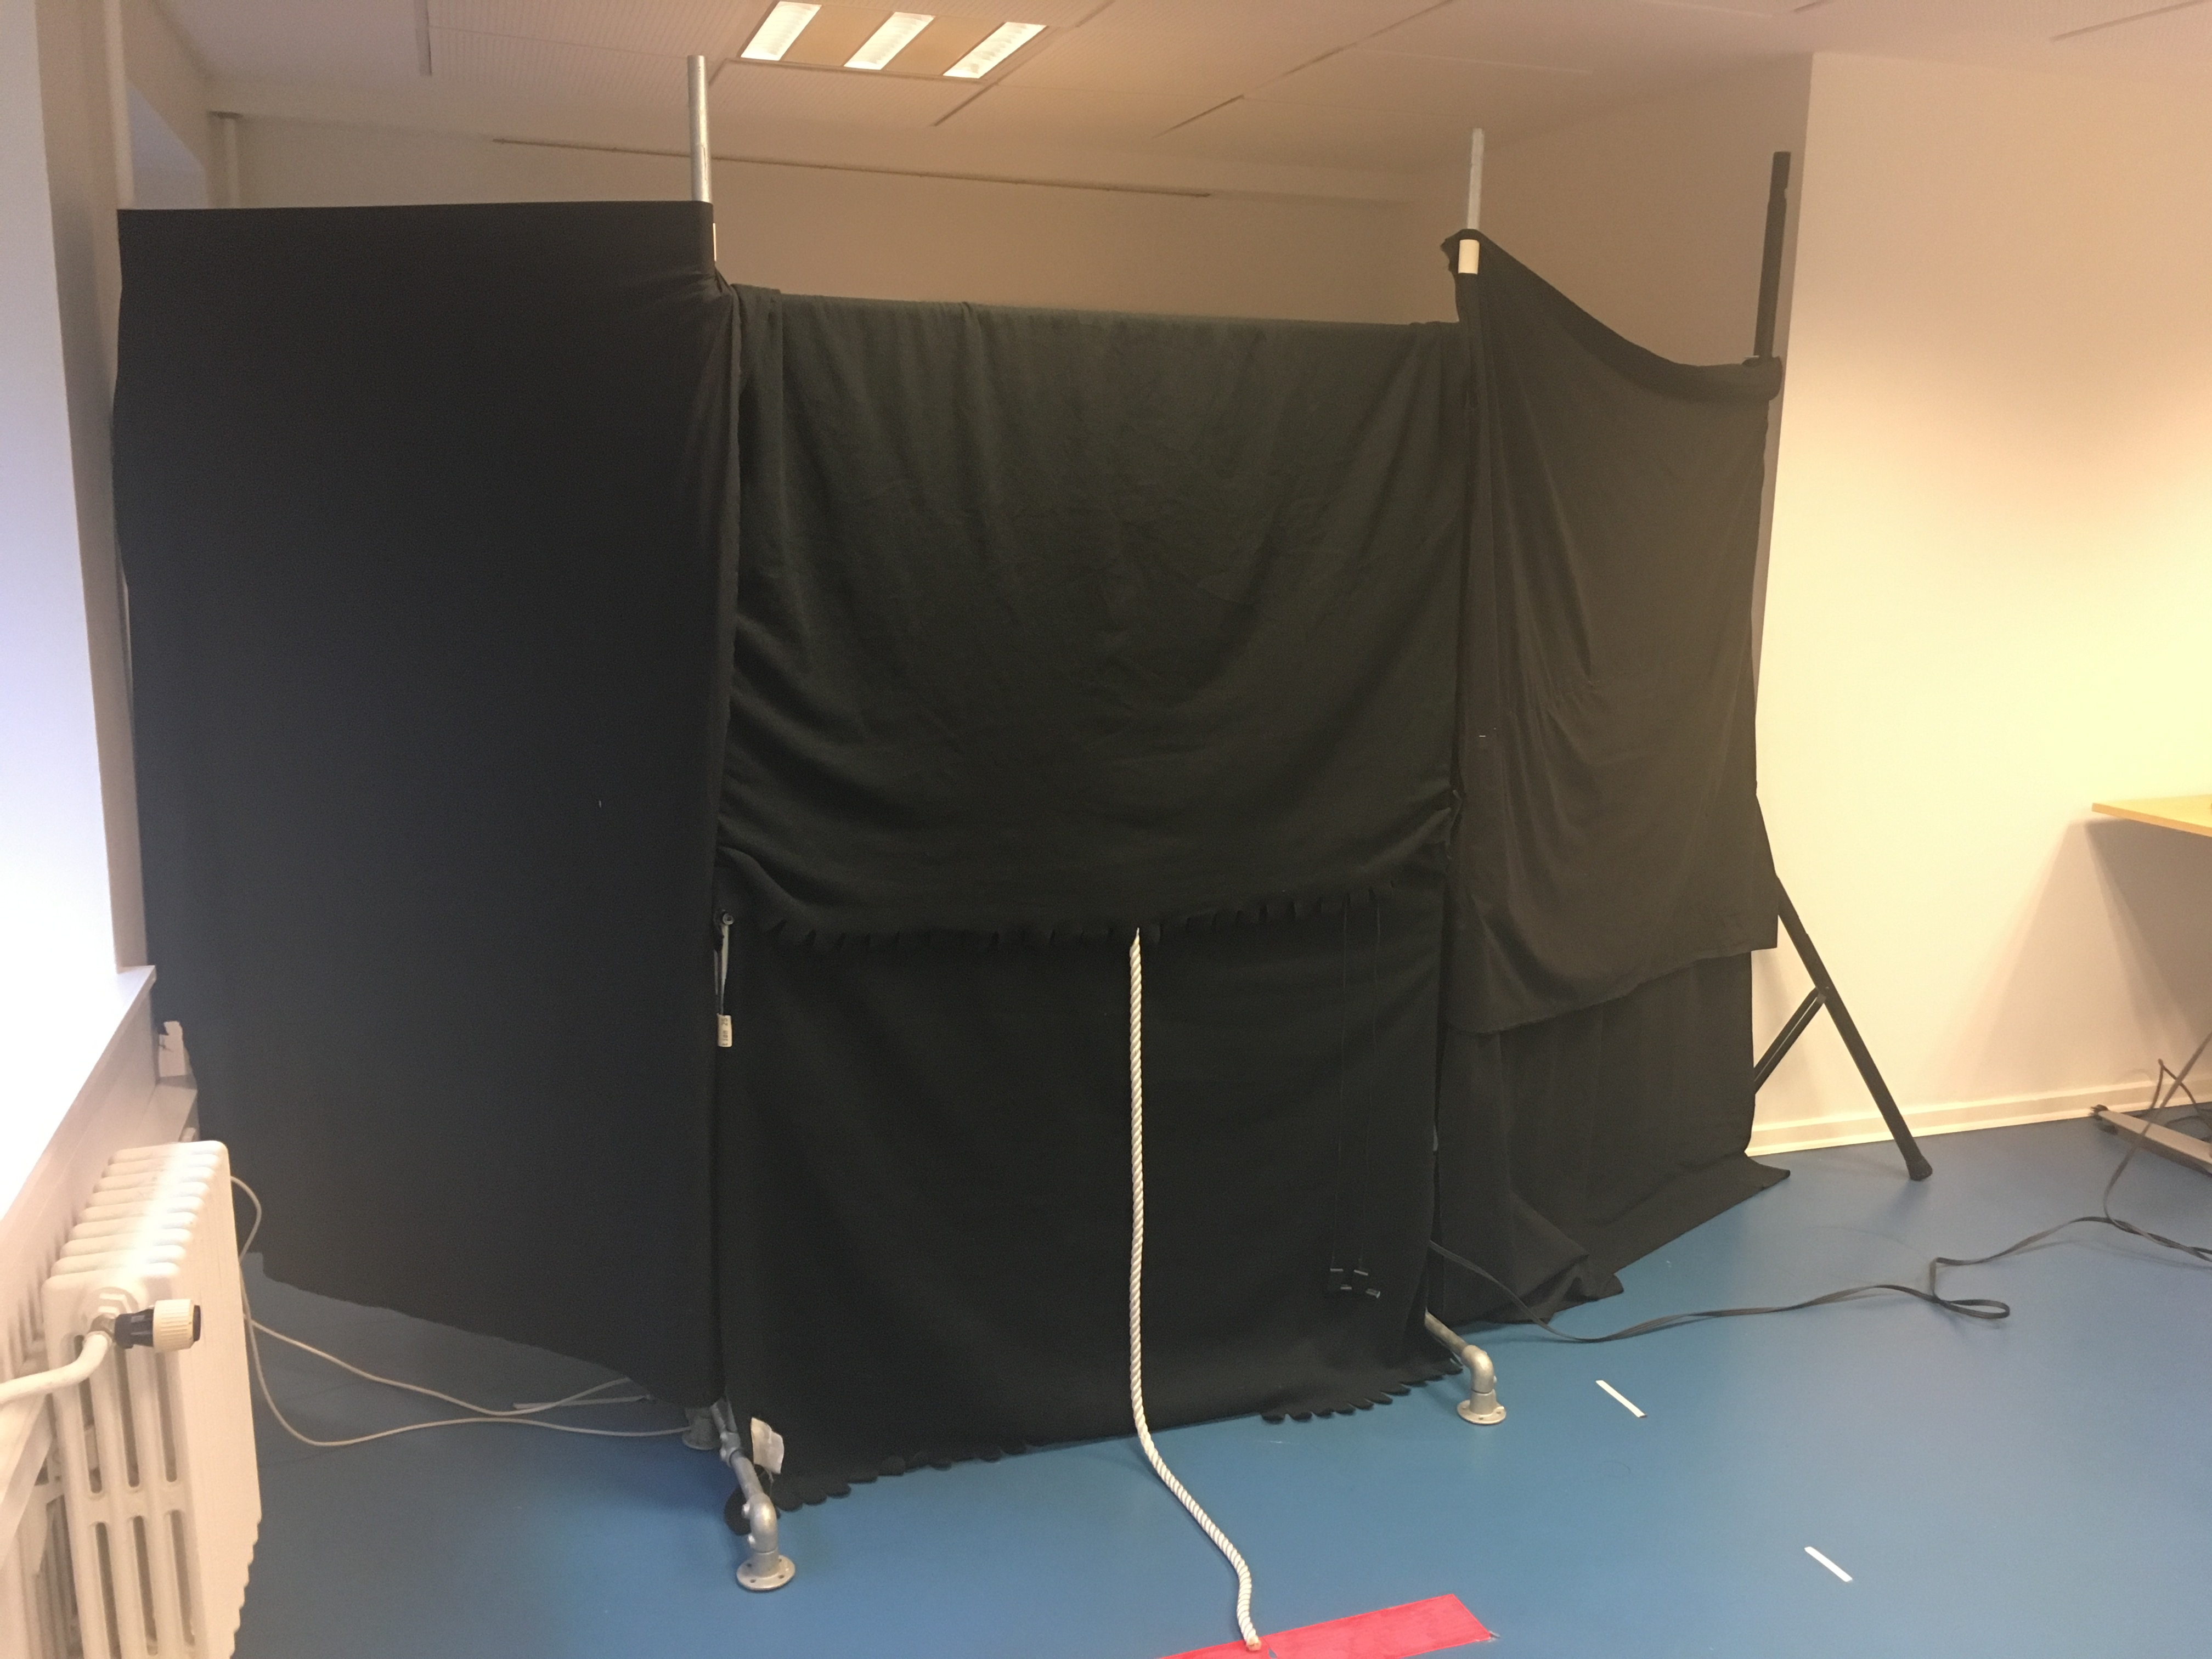
\includegraphics[width=\textwidth]{Images/setup1.JPG}
  \end{minipage}
  \hfill
  \begin{minipage}[b]{0.4\textwidth}
    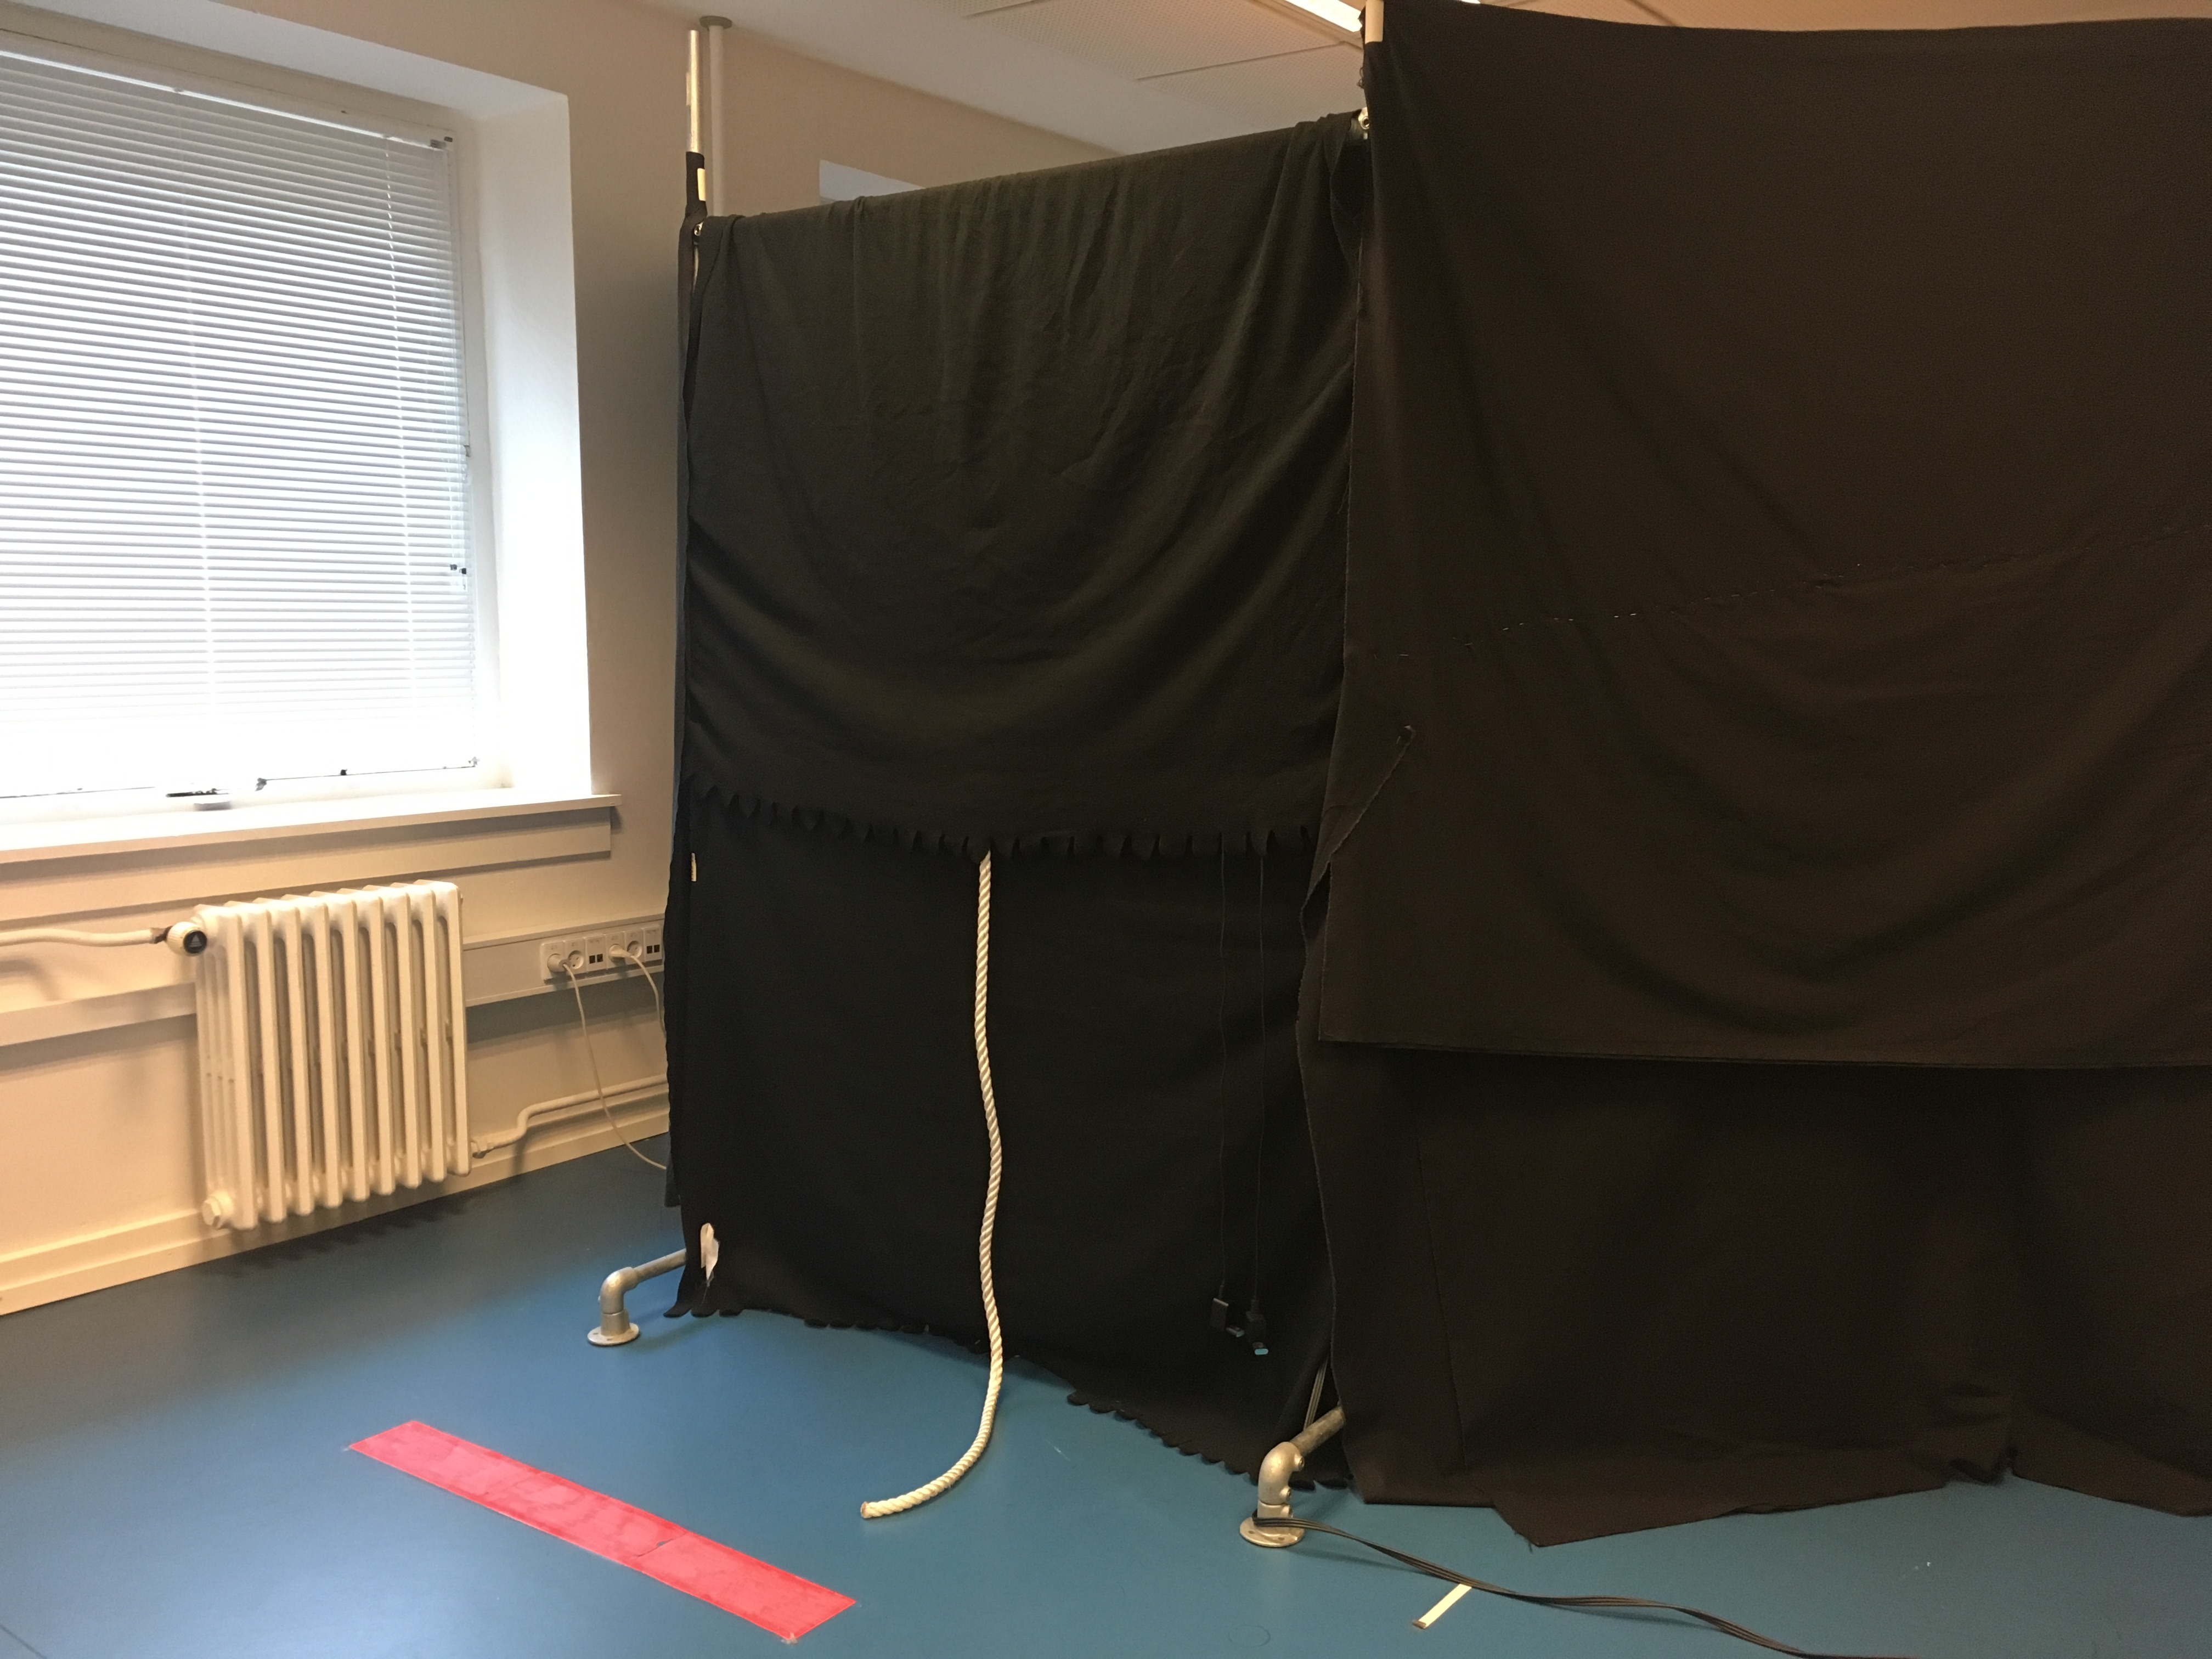
\includegraphics[width=\textwidth]{Images/setup2.JPG}
  \end{minipage}
\hspace*{\fill}
     \caption{Participants' view of the setup.}
     \label{fig:setupBlack}
\end{figure}
\begin{figure}
  \centering
  \captionsetup{justification=centering,margin=0.1cm}
\hspace*{\fill}
  \begin{minipage}[b]{0.4\textwidth}
    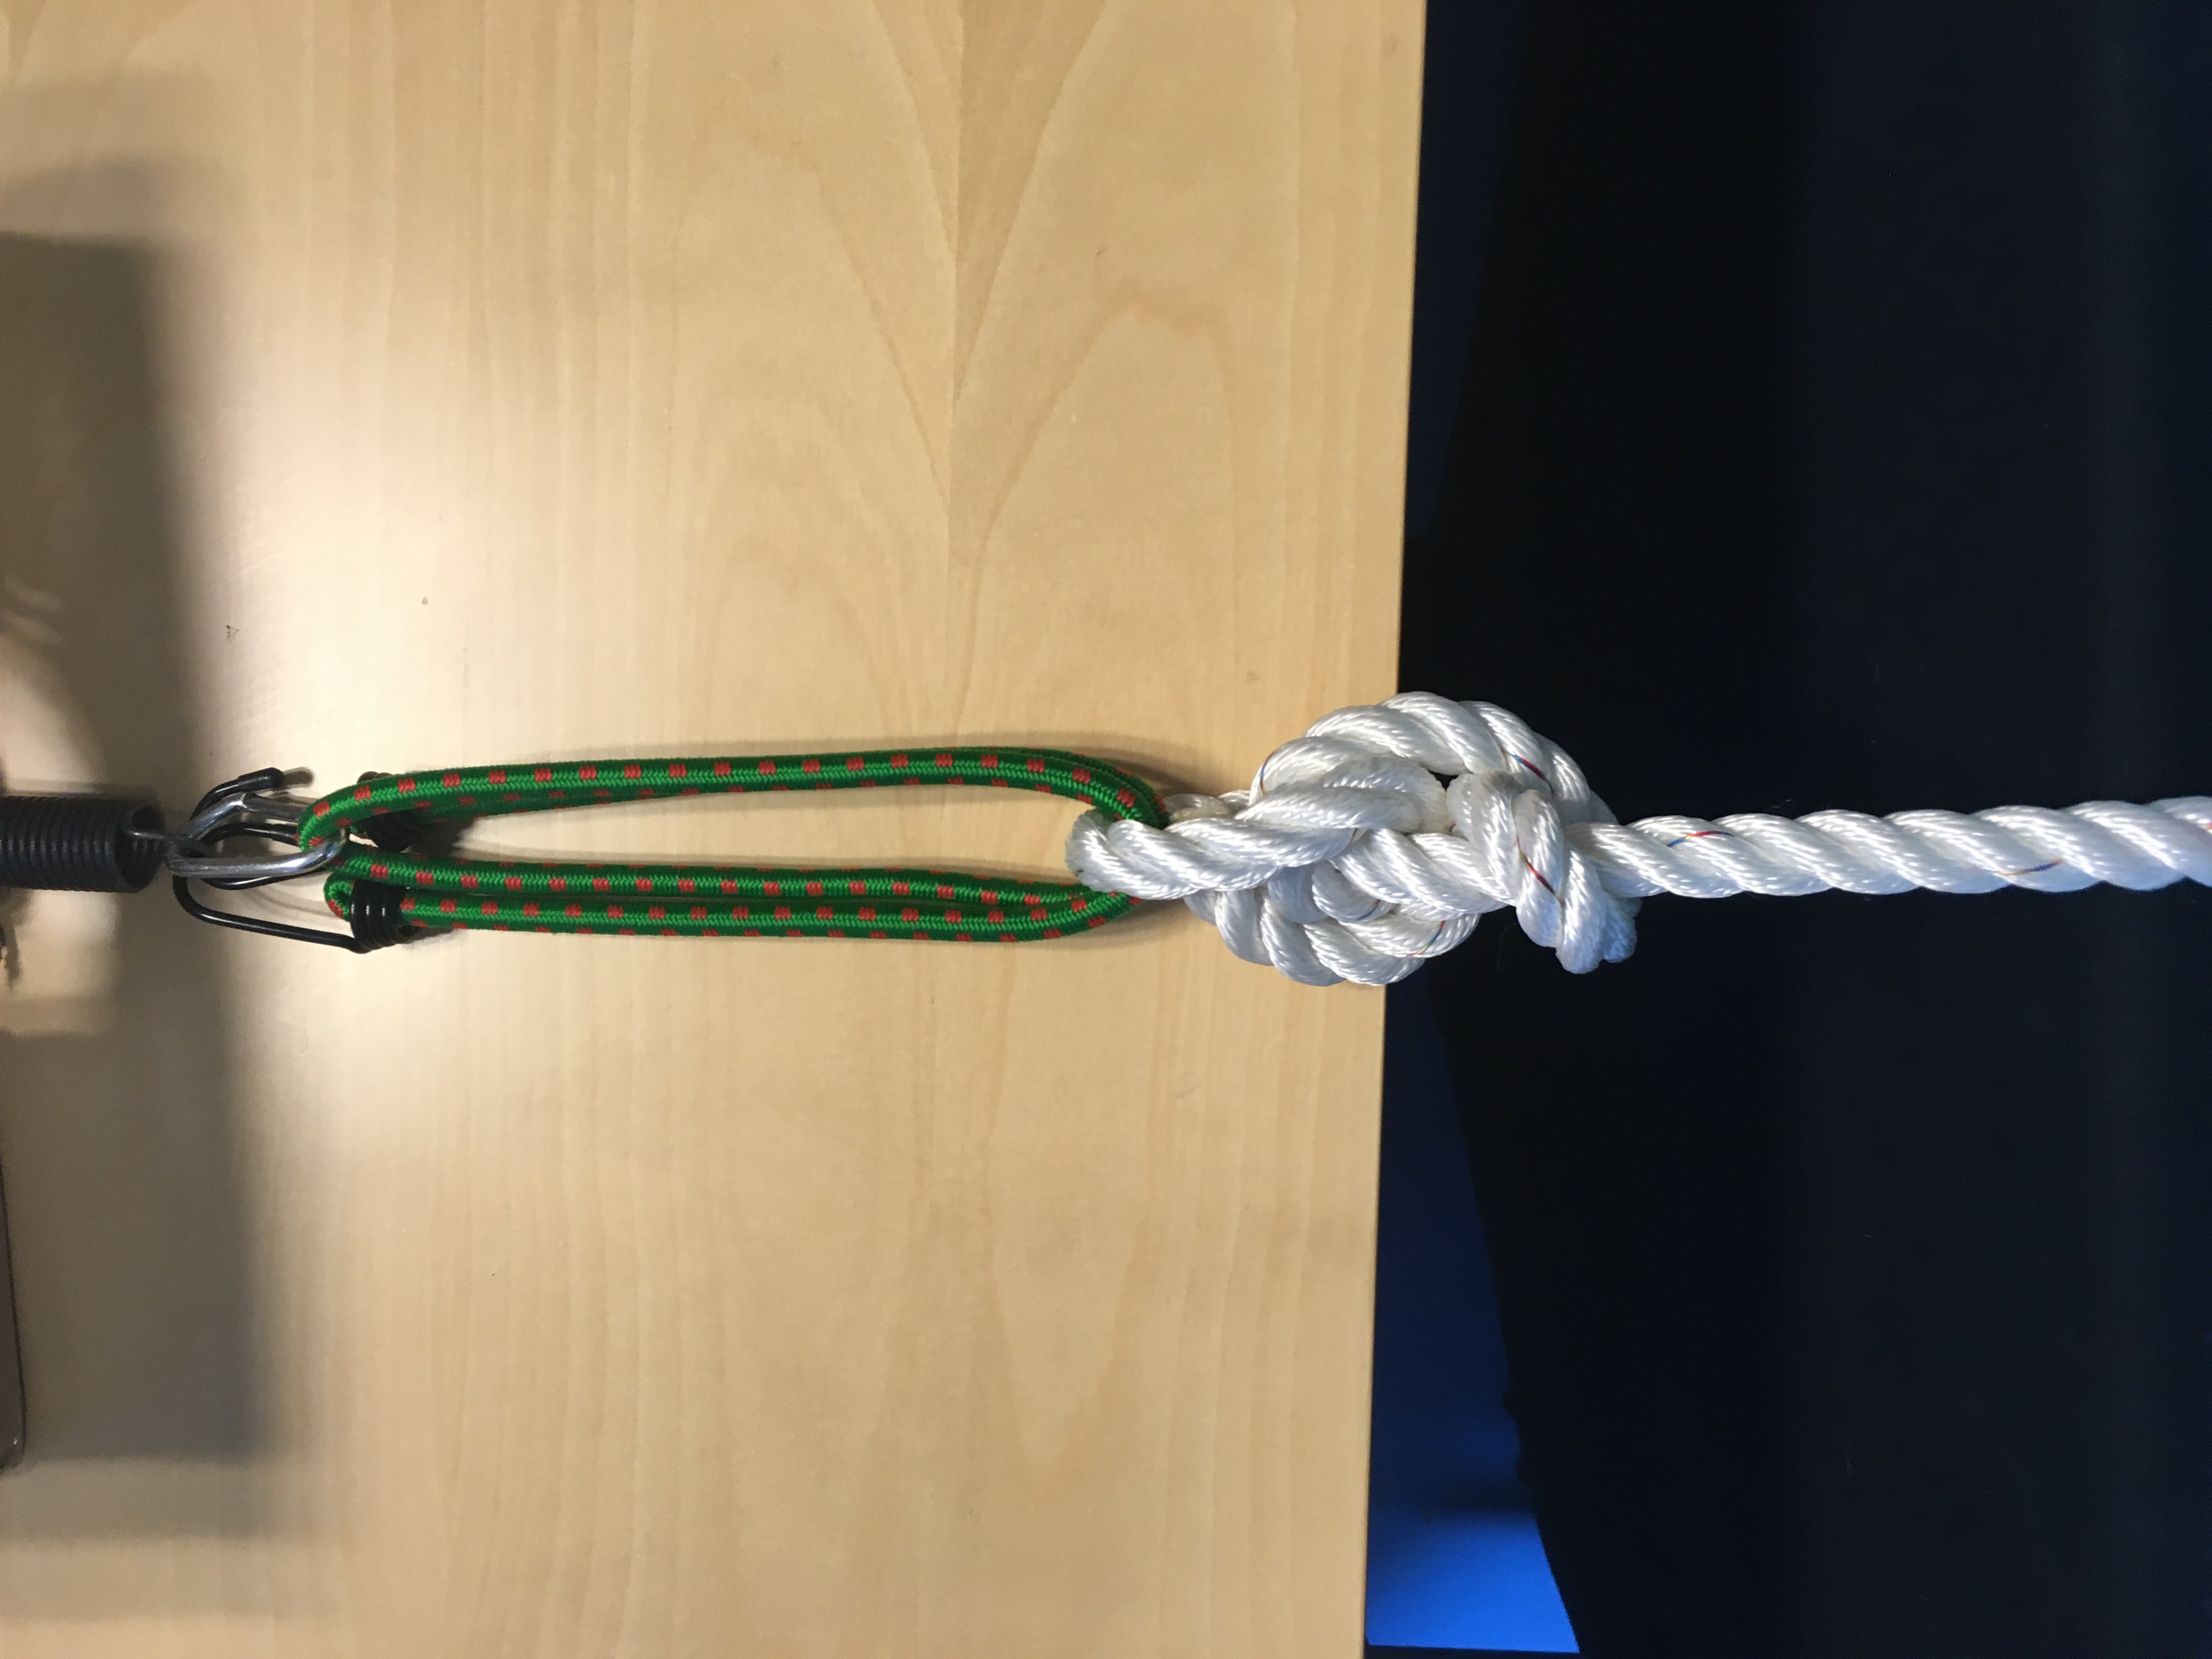
\includegraphics[width=\textwidth]{Images/rope.JPG}
    \caption{Rope and spring tied to the meter.}
     \label{fig:setupRopeBox1}
    \end{minipage}
  \hfill
  \begin{minipage}[b]{0.4\textwidth}
    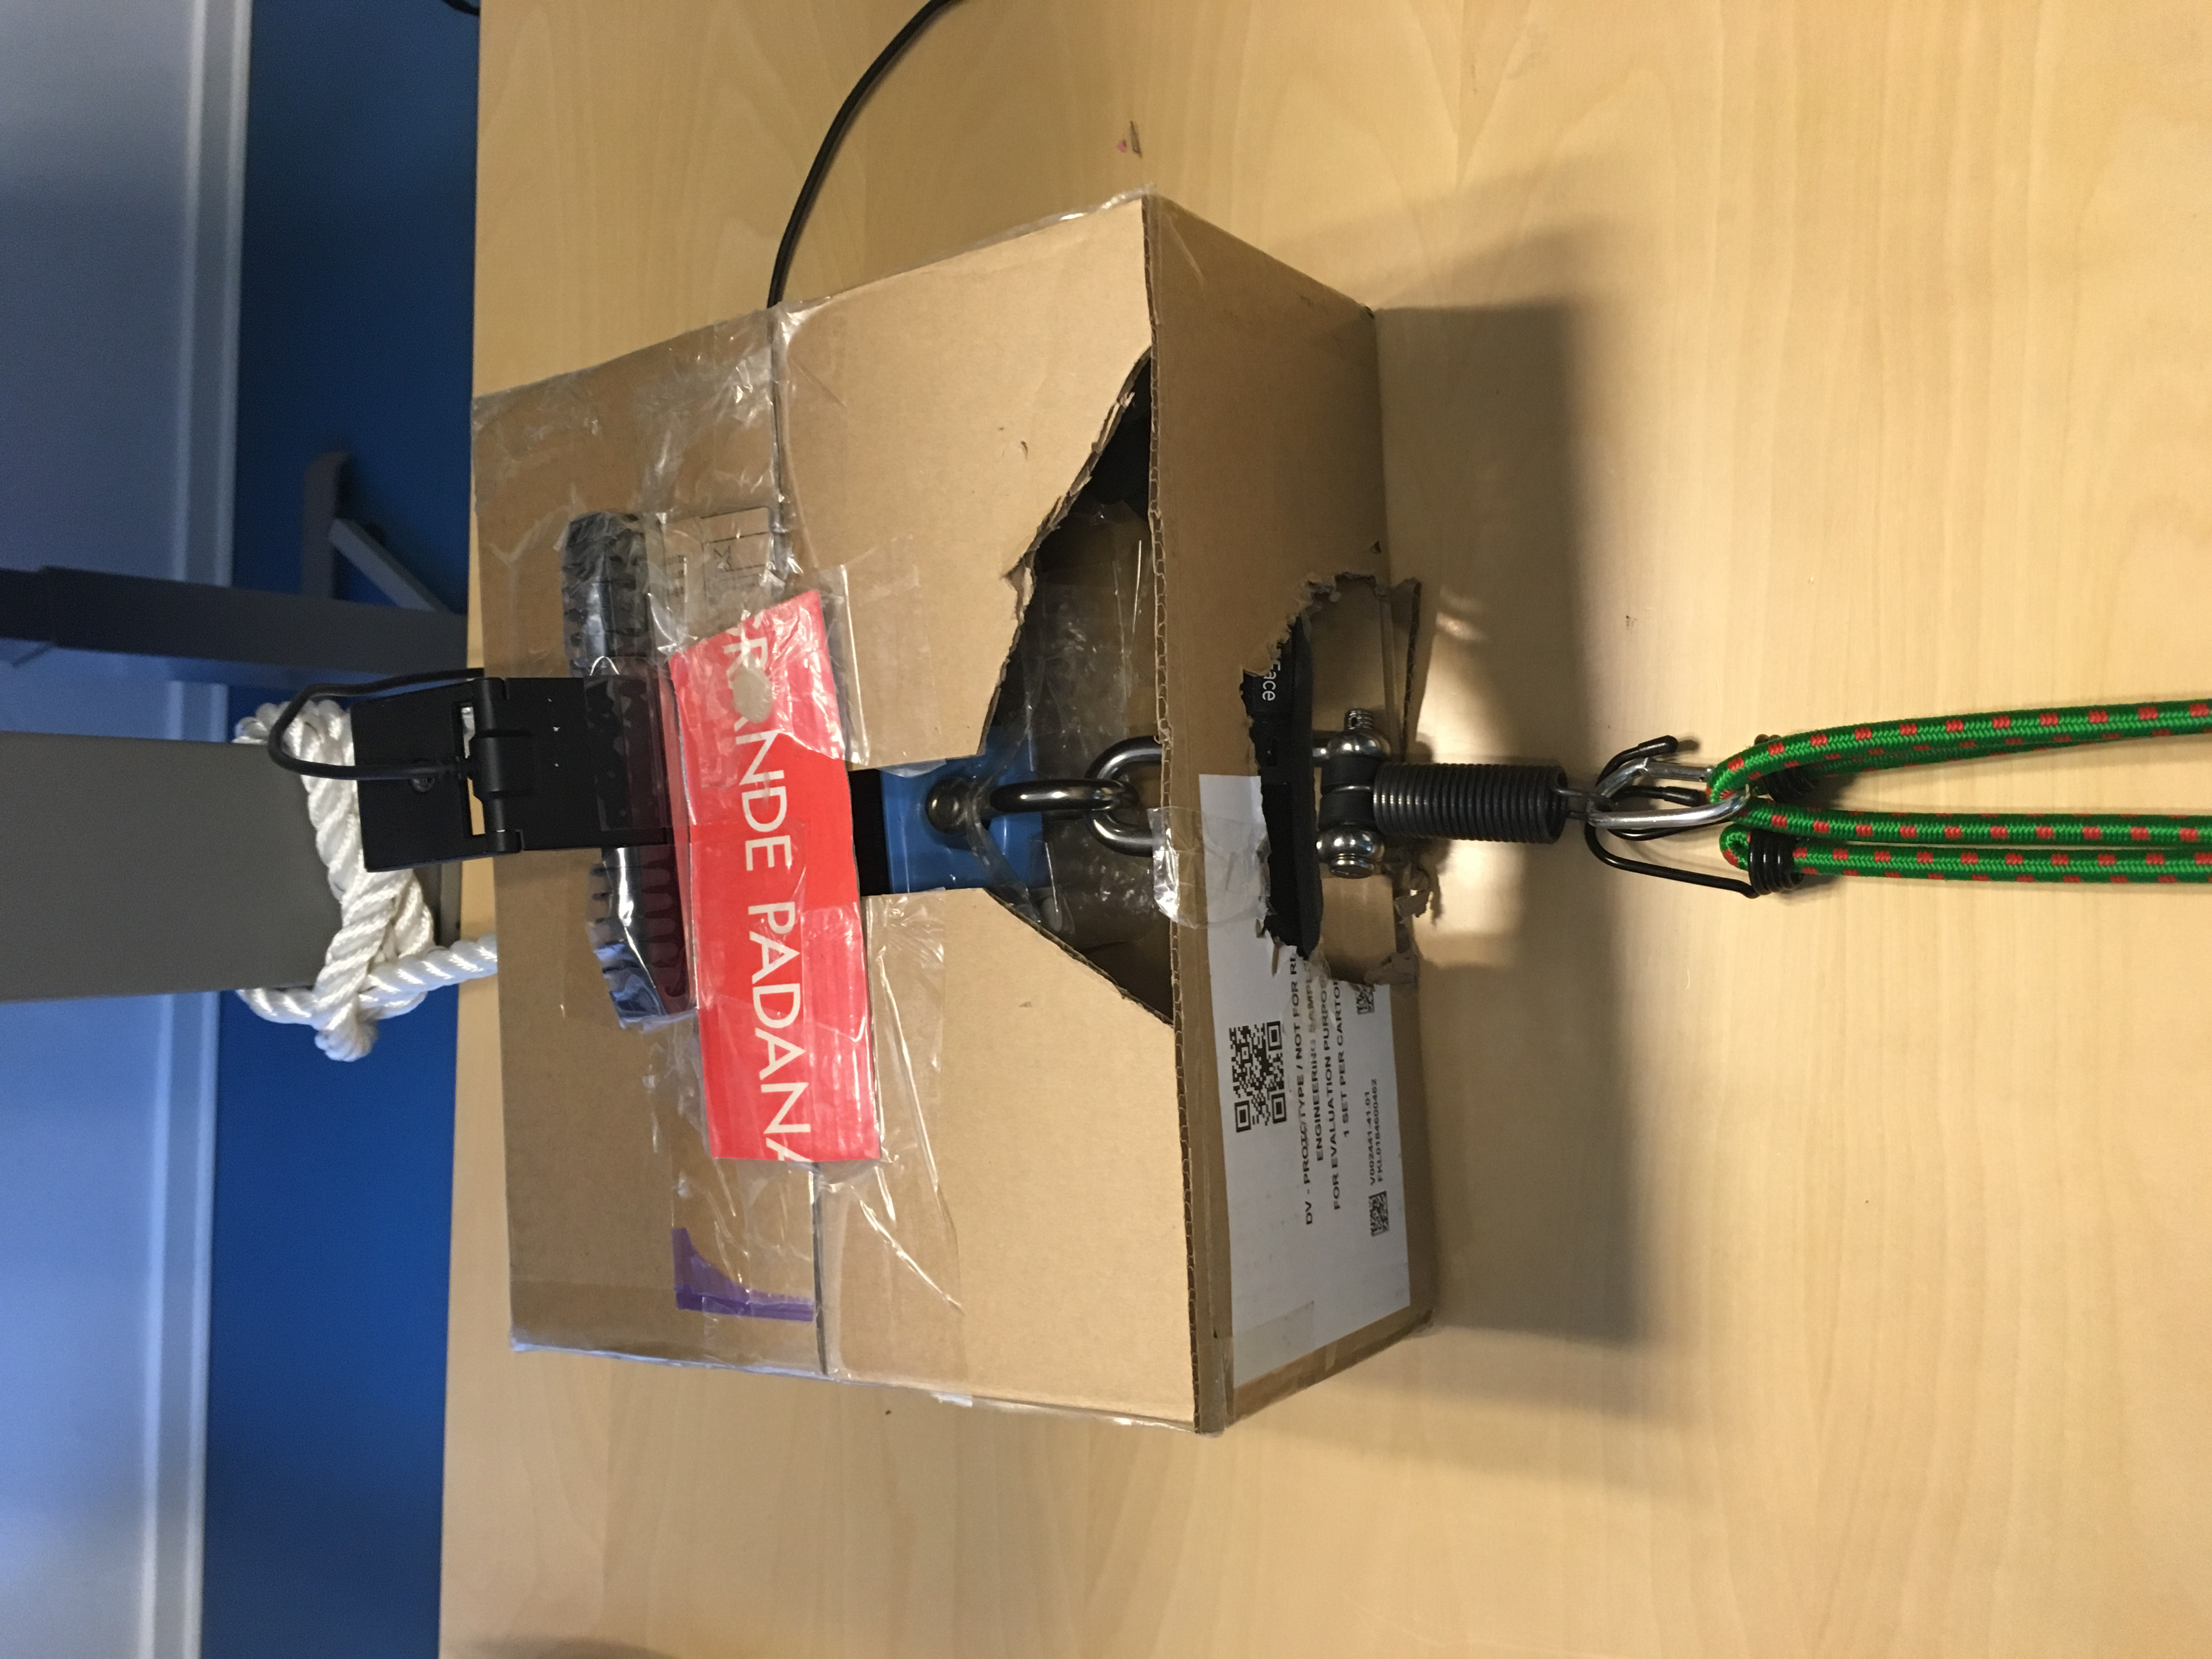
\includegraphics[width=\textwidth]{Images/BoxBig.JPG}
    \caption{Box with force meter and camera.}
     \label{fig:setupRopeBox2}
  \end{minipage}
\hspace*{\fill}
\end{figure}

\subsection{Procedure}
We greeted participants and briefly explained the broad purpose of the study. After that, we gave them two consent forms to fill in and further explained details and constraints of the tug-of-war game. Before giving participants the VR headset and gloves, they filled in a short survey with demographic data. The experimental procedure is fully explained in section \ref{subsection:instructionSheet}.
\\
Before starting the game, we calibrated the gloves for participants' hands. For each rope-pulling trial, participants were told to start pulling after the end of the countdown, when they they see \textit{Start}, and keep pulling until they see \textit{STOP}. They also received audio feedback for the countdown. Participants were told to follow two constraints: always keep their hands on the rope and try pulling the rope without moving their legs. Between rope-pulls, participants answered the questions on the quiz panel (figure \ref{fig:VRPanel}) from within the VE. After 5 rope-pulls, the game ends and participants are asked to fill in the post-experimental survey. The survey questions of the avatar appearances were gender-matched. Before participants left, we collected feedback about the game and then debriefed users about the true scope of the study.\\
For each trial, users pulled the rope for 10 seconds. Before that, they were in the VE with their opponent for 20 seconds. After the pulling ended, they remained in the same VR state for an additional 10 seconds. During this time, users could inspect the appearance of the avatars. Only after that, participants were shown the quiz panel. Transition between the game states (rope-pulling and quiz panel) was realized through a black splash screen. When the screen faded to black, the objects in the room changed. The screen fades back when the changes are complete. We did this in order to maintain a natural state of the room and prevent breaks in presence and immersion. Further details about the implementation are presented in section \ref{section:implementation}.\\
\subsection{Participants}
\label{subsection:participantsExperiment}
In order to give the appearance of a gaming study, we designed a poster to recruit people for the experiment. We placed this poster (\ref{subsection:poster}) around the university campus and  used it for recruiting messages. For the user study, we recruited a total of 28 participants (17 female) from the university campus and local Facebook groups. They were between 21 and 34 years old $(M = 24.42, SD = 3.06)$. Participants were unable to take part in the study if they previously completed the avatar appearance survey. We discarded the results of 2 participants (1 female) due to invalid data. Of the remaining ones, 9 participants had never used VR before and 16 had never played real-life tug-of-war. Participants were rewarded with a gift valued at 100 danish krone for taking part in the whole study.
\subsection{Results}
The results were manually logged by the experimenter. To measure the maximum force, we looked at the force meter data from the end of the countdown, at the beginning of the \textit{START} message, until the end of the \textit{STOP} message. In the plots below, we present data in terms of ordering and condition. By ordering, we mean the order in which participants saw the appearances, labeled as \textit{Trial}. By condition we mean the condition of the opponent participants faced, labeled as \textit{Condition}. Trial 1 refers to the first trial of rope-pulling participants performed, out of a total of five. Trial 2 refers to the second one and so on. The condition captures the independent variable and represents a numerical mapping from 1 to 5 to the appearance variable, increasing by strength/intimidation. Condition 1 refers to the weakest looking chosen avatar according to the weighted score (see \ref{fig:SurveyRatedFemalesChosen},\ref{fig:SurveyRatedMalesChosen}) and condition 5 refers to the strongest looking avatars. We also display our results by gender.
\subsubsection{Conditions per Trial}
\begin{figure}[H]
\vspace*{-3mm}
 \centering
 \captionsetup{justification=centering,margin=0.1cm}
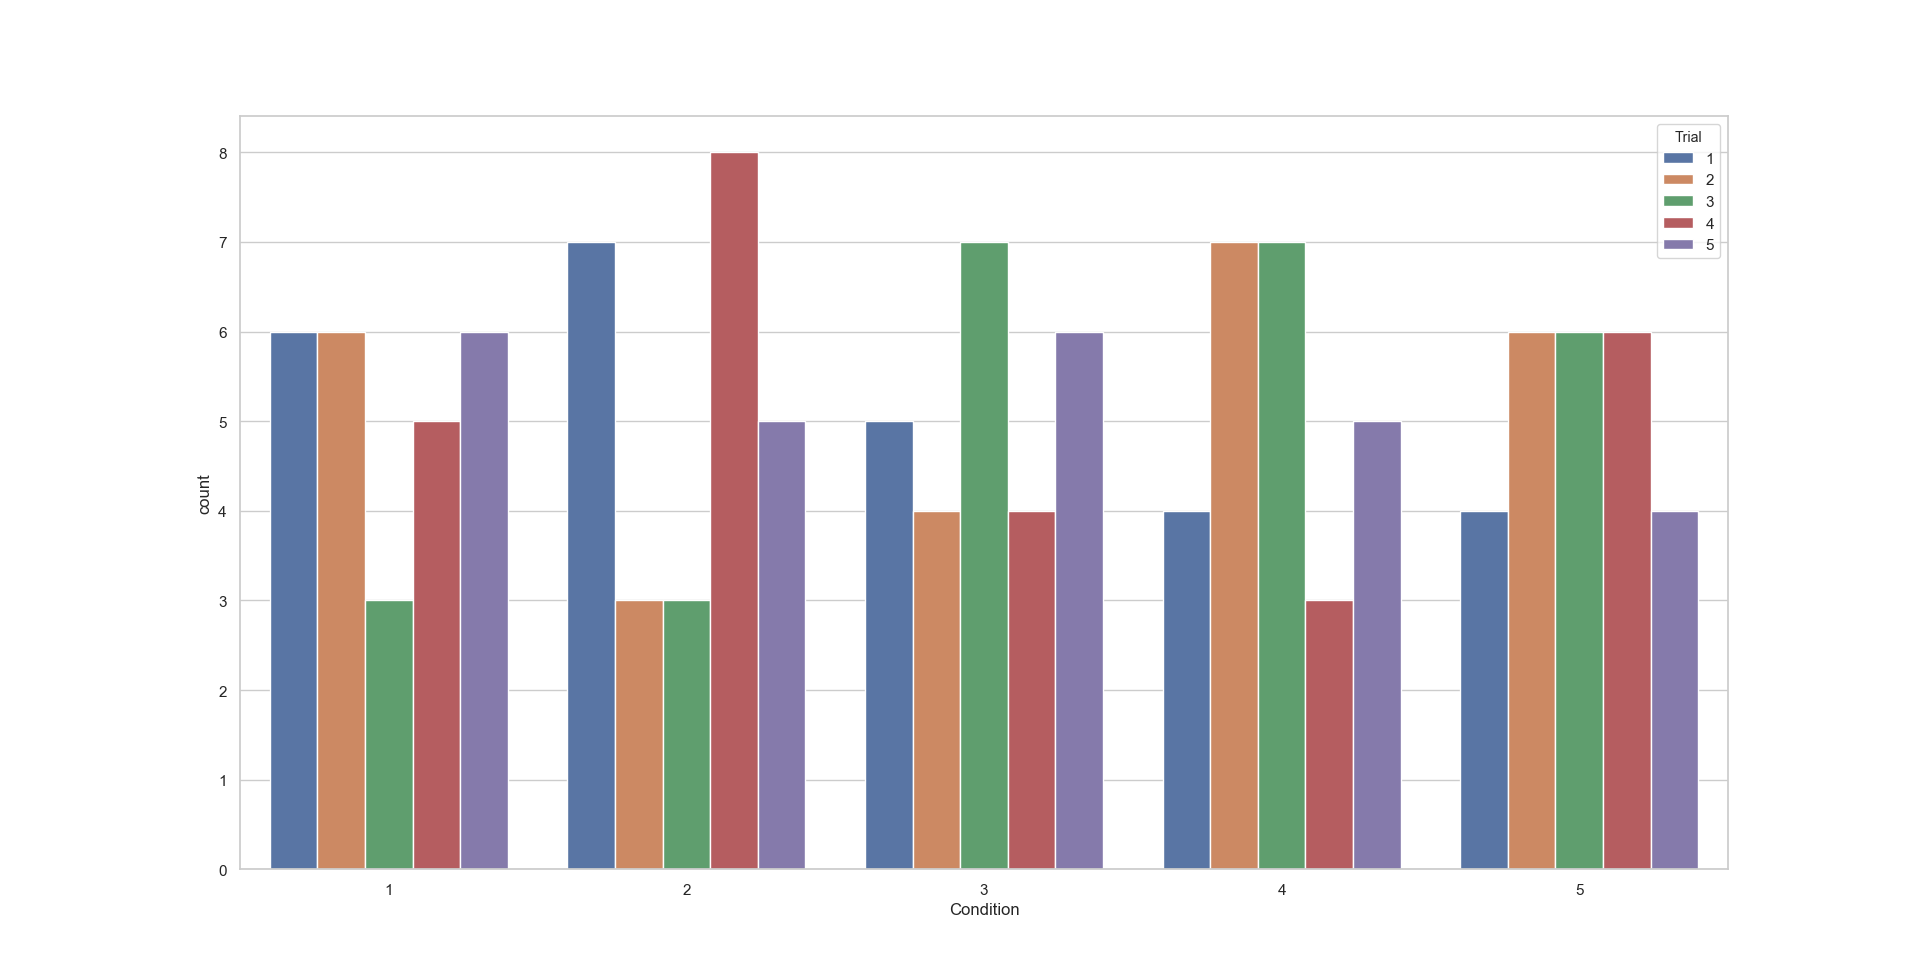
\includegraphics[width=0.9\textwidth]{Files/Plots/condition_by_trial.png}
 \caption{Number of conditions per trial.}
 \label{fig:condPerTrial}
  \end{figure}
\begin{figure}[H]
\vspace*{-10mm}
\centering
\captionsetup{justification=centering,margin=0.1cm}
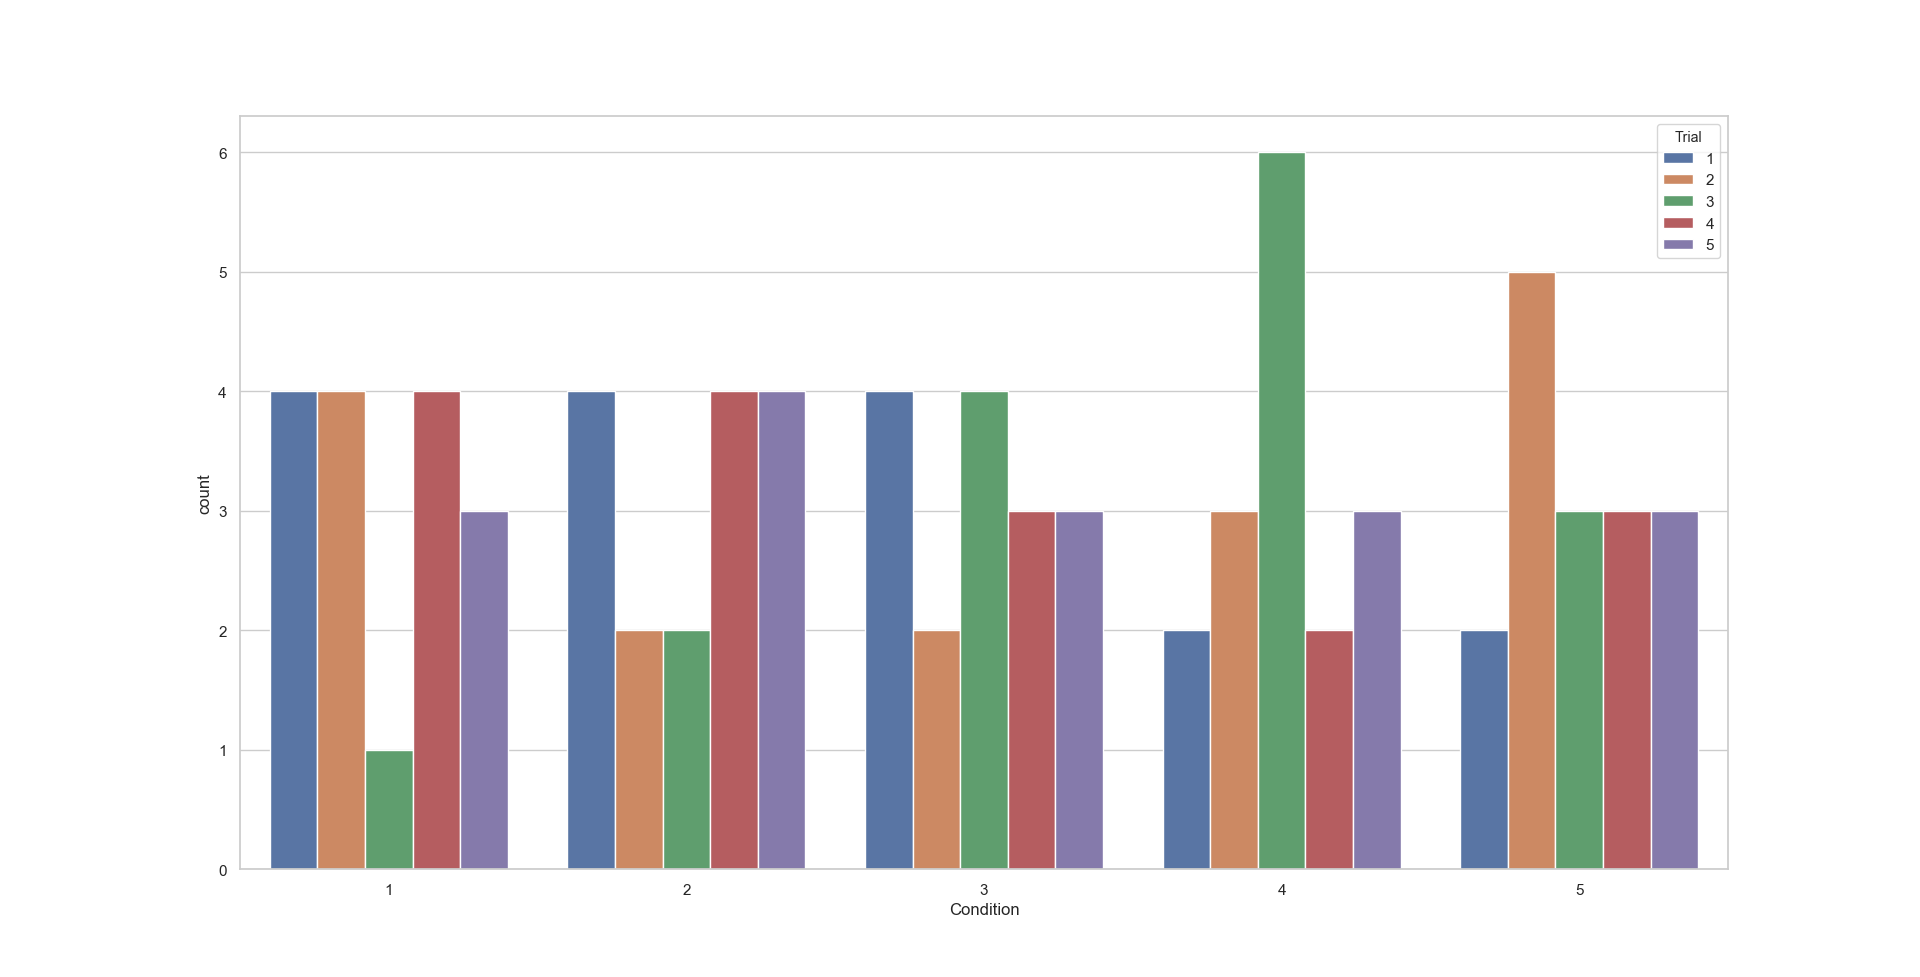
\includegraphics[width=0.9\textwidth]{Files/Plots/condition_by_trial_females.png}
 \caption{Number of conditions per trial for females.}
 \label{fig:condPerTrialF}
\end{figure}

\begin{figure}[H]
\vspace*{-10mm}
\centering
\captionsetup{justification=centering,margin=0.1cm}
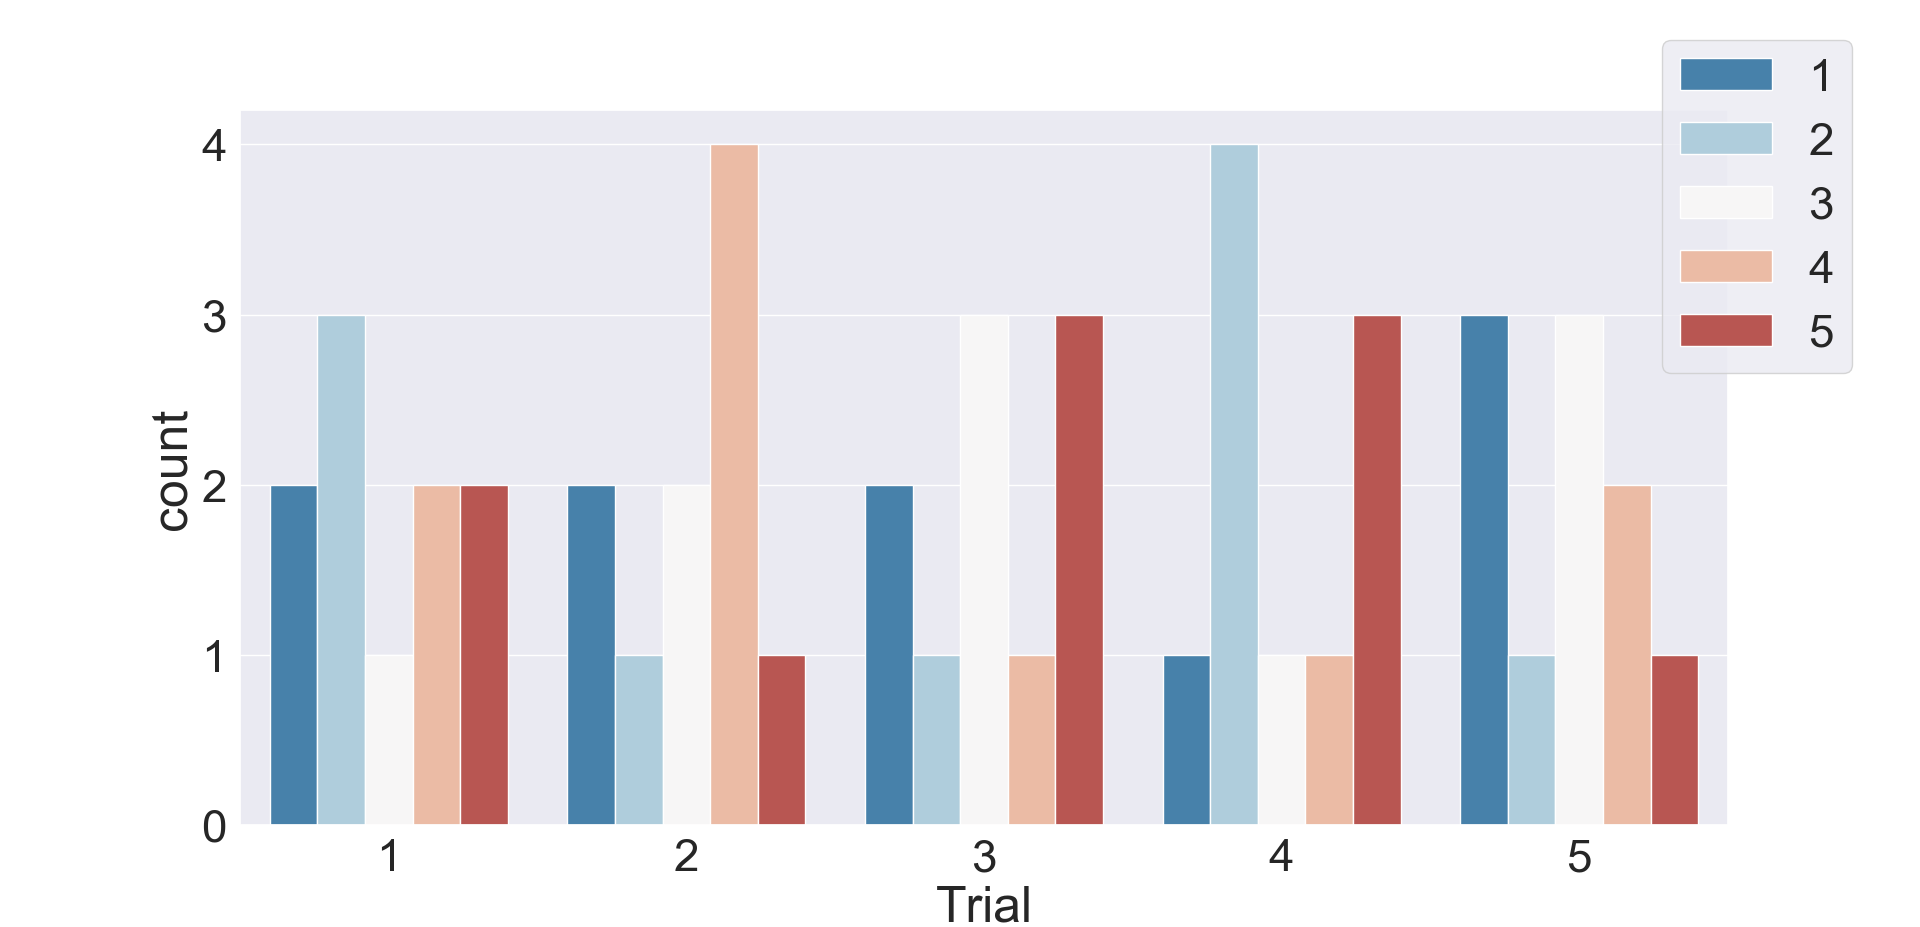
\includegraphics[width=0.9\textwidth]{Files/Plots/condition_by_trial_males.png}
\caption{Number of conditions per trial for males.}
\label{fig:condPerTrialM}
\end{figure}
In the above pictures we show the distribution of each condition for each trial. Since the conditions were randomized there may be an effect of over-representation.

\subsubsection{Appearance Ratings}
\begin{figure}[H]
 \hspace*{\fill}
     \begin{subfigure}[b]{0.4\textwidth}
         \centering
         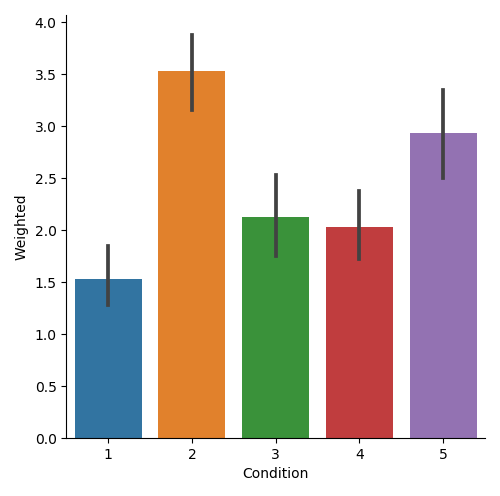
\includegraphics[width=\textwidth]{Files/Plots/weighted_ratings_female_experiment.png}
         \caption{Ratings for female avatars.}
         \label{fig:weightedFEx}
     \end{subfigure}
      \hspace*{\fill}
     \begin{subfigure}[b]{0.4\textwidth}
         \centering
         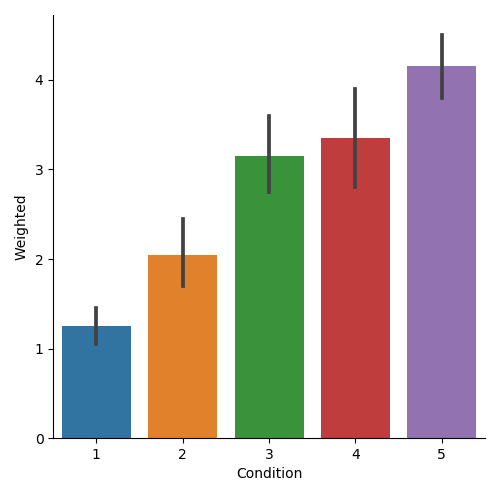
\includegraphics[width=\textwidth]{Files/Plots/weighted_ratings_male_experiment.png}
         \caption{Ratings for male avatars.}
         \label{fig:weightedMEx}
     \end{subfigure}
      \hspace*{\fill}
     \caption{Weighted ratings by condition for the opponent avatars in the user study.}
         \label{fig:weightedEX}
\end{figure} 
Participants rated the appearance of same-gender avatars on attractiveness, intimidation, intelligence and strength. In the above  figures we present the weighed results of those ratings for female (\ref{fig:weightedFEx}) and male (\ref{fig:weightedMEx}) avatars. The weighted value is computed as $weighted=0.5strength+0.5intimidation$.
Male participants rated the avatars as expected, increasing in intimidation and strength by condition. For females, the avatar in condition 2 (low-average) was rated as highest in intimidation and strength, while the avatar in condition 5 (strong) came second. All ratings for these avatars and their thumbnails can be found in section \ref{subsection:thumbnailsExperiment}. 

\subsubsection{Force Meter Results}
\begin{figure}[H]
\hspace*{\fill}
     \begin{subfigure}[b]{0.4\textwidth}
         \centering
         \vspace*{-10mm}
         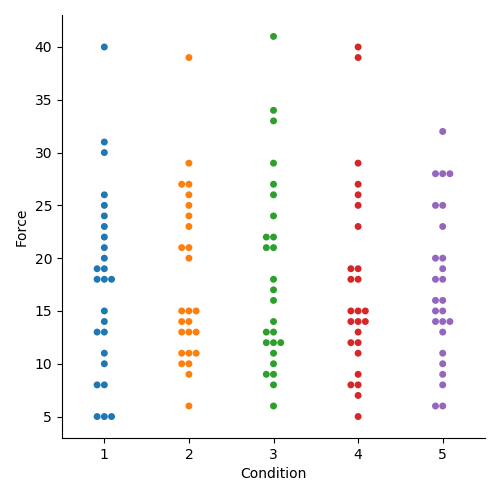
\includegraphics[width=\textwidth]{Files/Plots/force_by_cond_swarm.png}
         \caption{All force values by condition.}
         \label{fig:allForceSwarm}
     \end{subfigure}
     \hspace*{\fill}
     \begin{subfigure}[b]{0.4\textwidth}
         \centering
         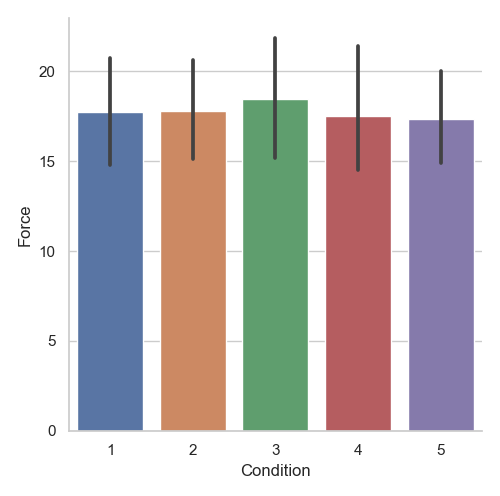
\includegraphics[width=\textwidth]{Files/Plots/force_mean_by_condition.png}
         \caption{Mean force by condition}
         \label{fig:allForceMeanCond}
     \end{subfigure}          
     \hspace*{\fill}
     \begin{subfigure}[b]{0.4\textwidth}
         \centering
         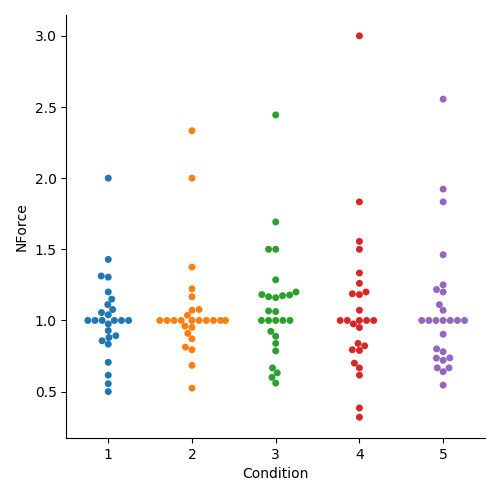
\includegraphics[width=\textwidth]{Files/Plots/forceNforce_by_cond_swarm.png}
         \caption{All N1 by condition. }
         \label{fig:allForceNCond}
     \end{subfigure}
     \hspace*{\fill}
     \begin{subfigure}[b]{0.4\textwidth}
         \centering
         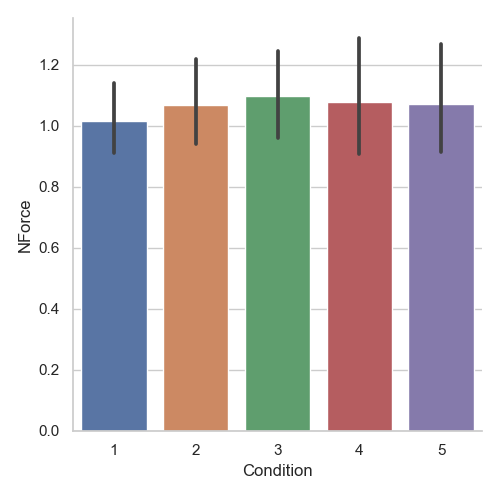
\includegraphics[width=\textwidth]{Files/Plots/forceNforce_mean_by_condition.png}
         \caption{Mean of N1  by condition. }
         \label{fig:allForceNCond}
     \end{subfigure} 
     \hspace*{\fill}
         \begin{subfigure}[b]{0.4\textwidth}
         \centering
         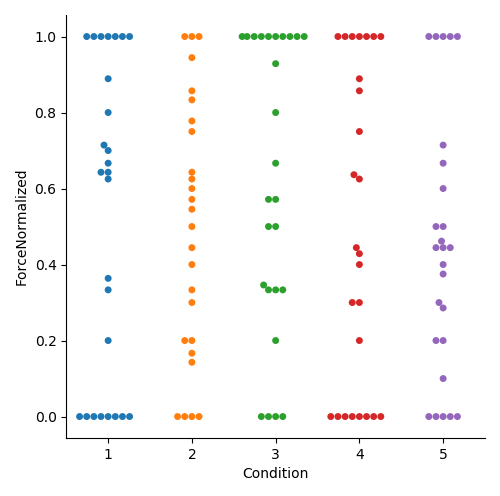
\includegraphics[width=\textwidth]{Files/Plots/forceNormalized_by_cond_swarm.png}
         \caption{All N2 by condition.}
         \label{fig:allForceNorm}
     \end{subfigure}
\hspace*{\fill}
     \begin{subfigure}[b]{0.4\textwidth}
         \centering
         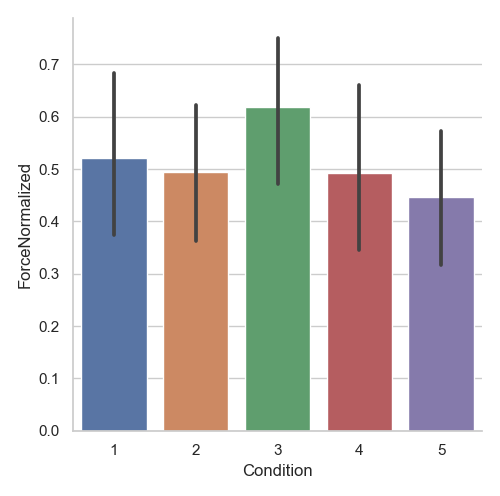
\includegraphics[width=\textwidth]{Files/Plots/forceNormalized_mean_by_condition.png}
         \caption{Mean of N2 by condition.}
         \label{fig:allForceNormMean}
     \end{subfigure} 
     
      \caption{All force values by condition. Lines on bars denote confidence intervals.}
         \label{fig:allForceCond}
\end{figure} 
\begin{figure}[H]
     \begin{subfigure}[b]{0.3\textwidth}
         \centering
         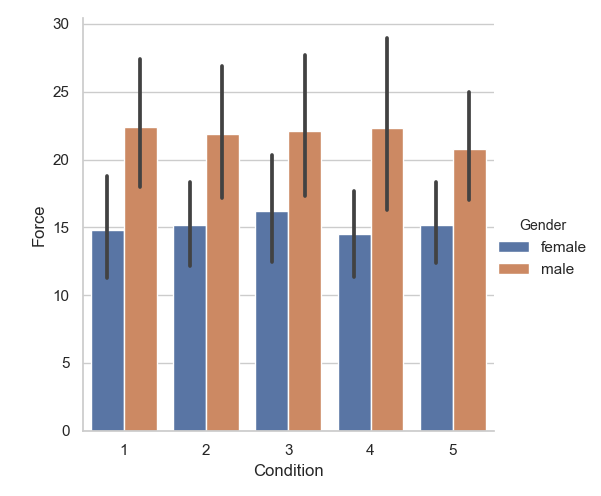
\includegraphics[scale=0.4]{Files/Plots/force_mean_by_condition__gen.png}
         \caption{Mean force.}
         \label{fig:forceMeanCondGen}
     \end{subfigure}
     \begin{subfigure}[b]{0.3\textwidth}
         \centering
         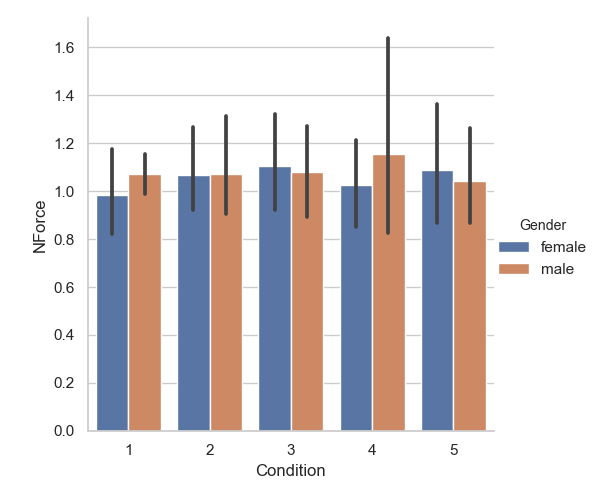
\includegraphics[scale=0.4]{Files/Plots/forceNforce_mean_by_condition_gen.png}
         \caption{Mean N1 force.}
         \label{fig:forceN1MeanGen}
     \end{subfigure}
      \begin{subfigure}[b]{0.3\textwidth}
         \centering
         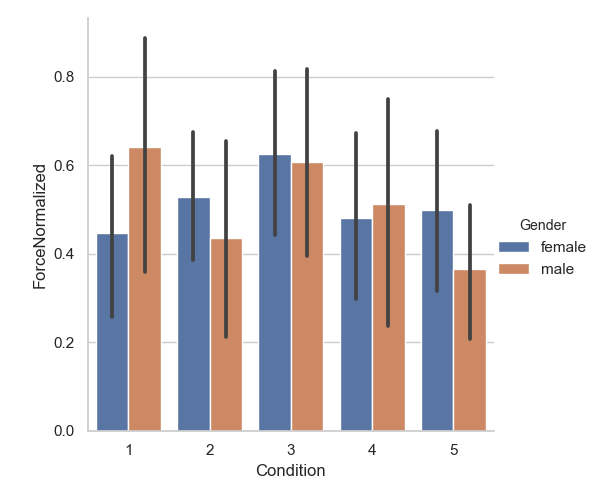
\includegraphics[scale=0.4]{Files/Plots/forceNormalized_mean_by_condition_gen.png}
         \caption{Mean N2 force.}
         \label{fig:forceN2MeanGen}
     \end{subfigure}
     \caption{Mean force, N1 , N2  by condition and by gender. Lines on bars denote confidence intervals.}
         \label{fig:forceMeanGenAll}
\end{figure} 


\begin{figure}[H]
     \begin{subfigure}[b]{0.3\textwidth}
         \centering
         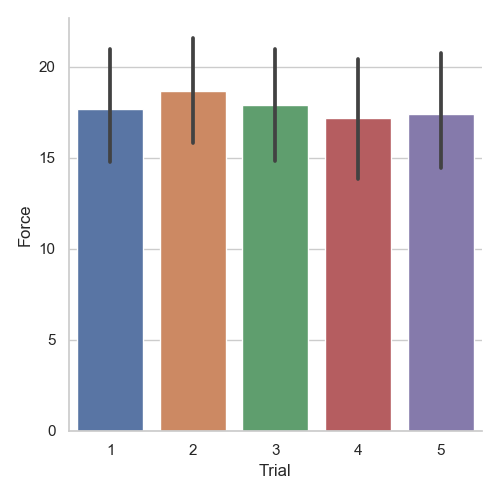
\includegraphics[scale=0.4]{Files/Plots/force_mean_by_trial.png}
         \caption{Mean force.}
         \label{fig:forceMeanTrial}
     \end{subfigure}
     \begin{subfigure}[b]{0.3\textwidth}
         \centering
         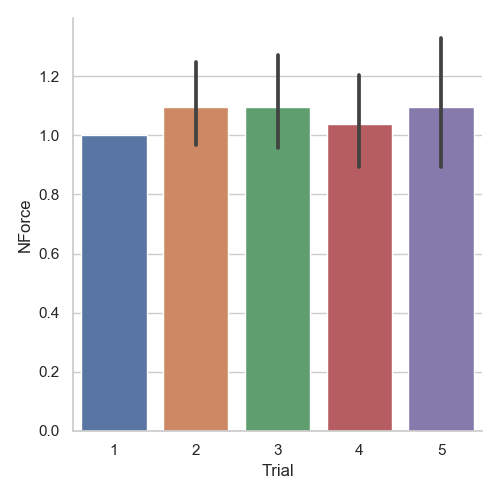
\includegraphics[scale=0.4]{Files/Plots/forceNforce_mean_by_trial.png}
         \caption{Mean N1 force.}
         \label{fig:forceN1Trial}
     \end{subfigure}
      \begin{subfigure}[b]{0.3\textwidth}
         \centering
         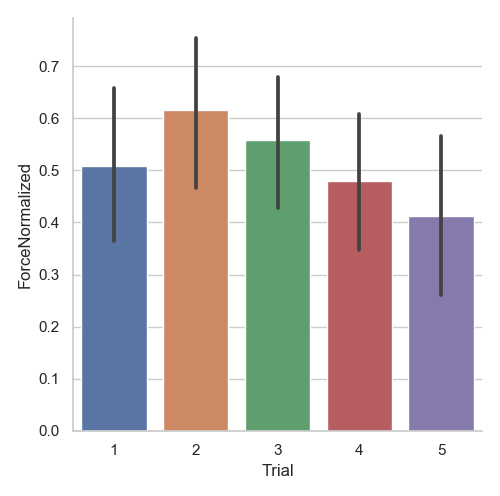
\includegraphics[scale=0.4]{Files/Plots/forceNormalized_mean_by_trial.png}
         \caption{Mean N2 force.}
         \label{fig:forceN2Trial}
     \end{subfigure}
         \begin{subfigure}[b]{0.3\textwidth}
         \centering
         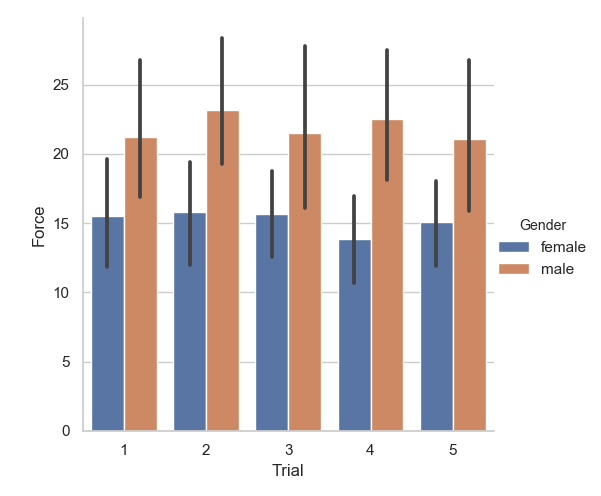
\includegraphics[scale=0.4]{Files/Plots/force_mean_by_trial_gen.png}
         \caption{Mean force.}
         \label{fig:forceMeanTrialGen}
     \end{subfigure}
     \begin{subfigure}[b]{0.3\textwidth}
         \centering
         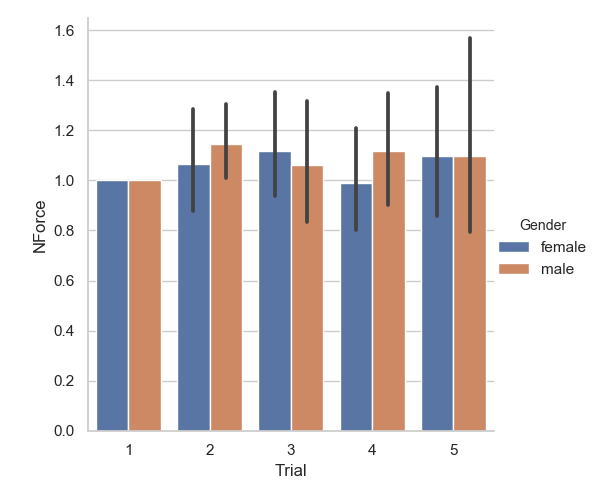
\includegraphics[scale=0.4]{Files/Plots/forceNforce_mean_by_trial_gen.png}
         \caption{Mean N1 force.}
         \label{fig:forceN1TrialGen}
     \end{subfigure}
      \begin{subfigure}[b]{0.3\textwidth}
         \centering
         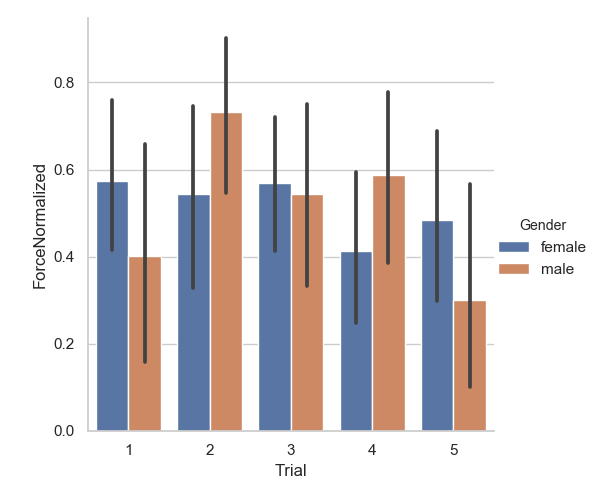
\includegraphics[scale=0.4]{Files/Plots/forceNormalized_mean_by_trial_gen.png}
         \caption{Mean N2 force.}
         \label{fig:forceN2TrialGen}
     \end{subfigure}
     \caption{Mean force, N1, N2  by trial, and by gender in the second row. Lines on bars are confidence intervals.}
         \label{fig:allForceTrial}
\end{figure} 

\begin{figure}[H]
 \begin{subfigure}[b]{0.5\textwidth}
     \centering
     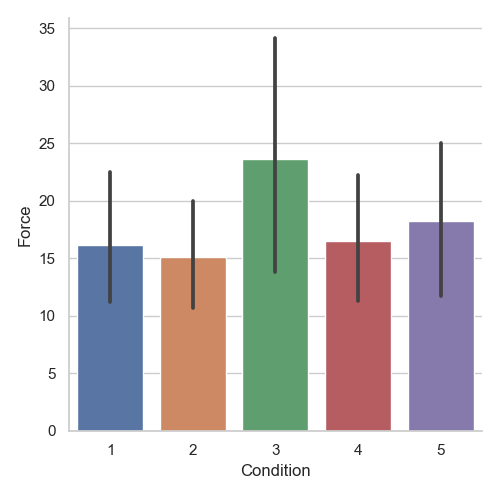
\includegraphics[scale=0.5]{Files/Plots/force_in_first_trial.png}
     \caption{Mean force in 1st trial.}
     \label{fig:meanF1st}
 \end{subfigure}
  \begin{subfigure}[b]{0.5\textwidth}
     \centering
     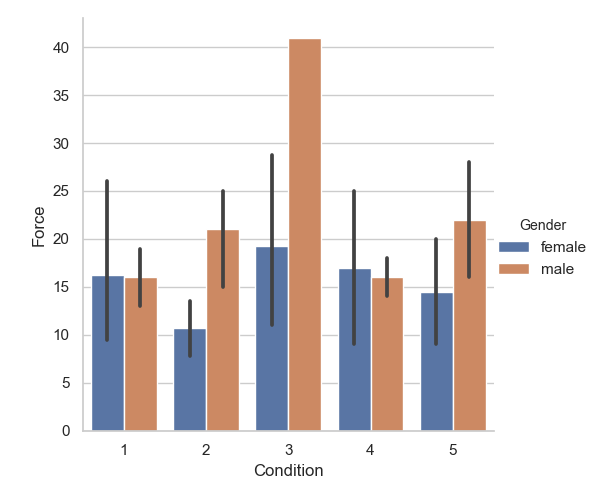
\includegraphics[scale=0.5]{Files/Plots/force_first_gen.png}
     \caption{Mean force in first trial gendered.}
     \label{fig:fig:meanF1stGen}
 \end{subfigure}
  \begin{subfigure}[b]{0.5\textwidth}
     \centering
     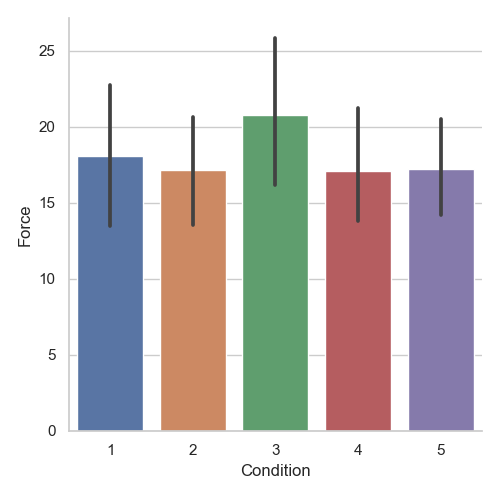
\includegraphics[scale=0.5]{Files/Plots/force_first_3.png}
     \caption{Mean force in first 3 trials.}
     \label{fig:fig:meanF3rd}
 \end{subfigure}
     \begin{subfigure}[b]{0.5\textwidth}
     \centering
     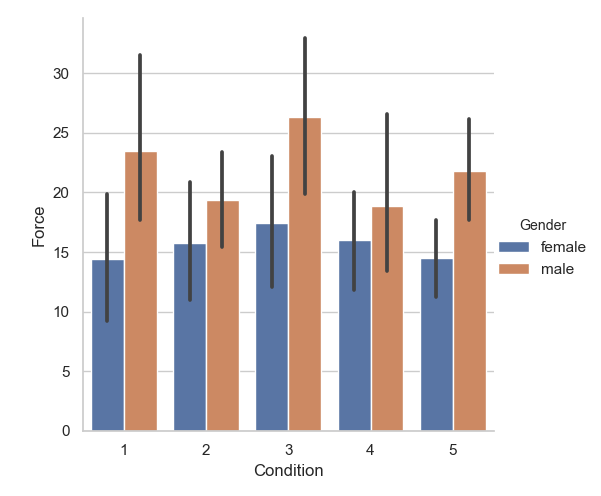
\includegraphics[scale=0.5]{Files/Plots/force_first_3_gen.png}
     \caption{Mean force in first 3 trials gendered.}
     \label{fig:fig:meanF3rdGen}
 \end{subfigure}
     \caption{Mean force by condition and by gender, taken for the first and first 3 trials. Lines on bars are confidence intervals.}
    \label{fig:forceIn1st3rd}
\end{figure}

\begin{figure}[H]
\hspace{-30mm}
 \centering
 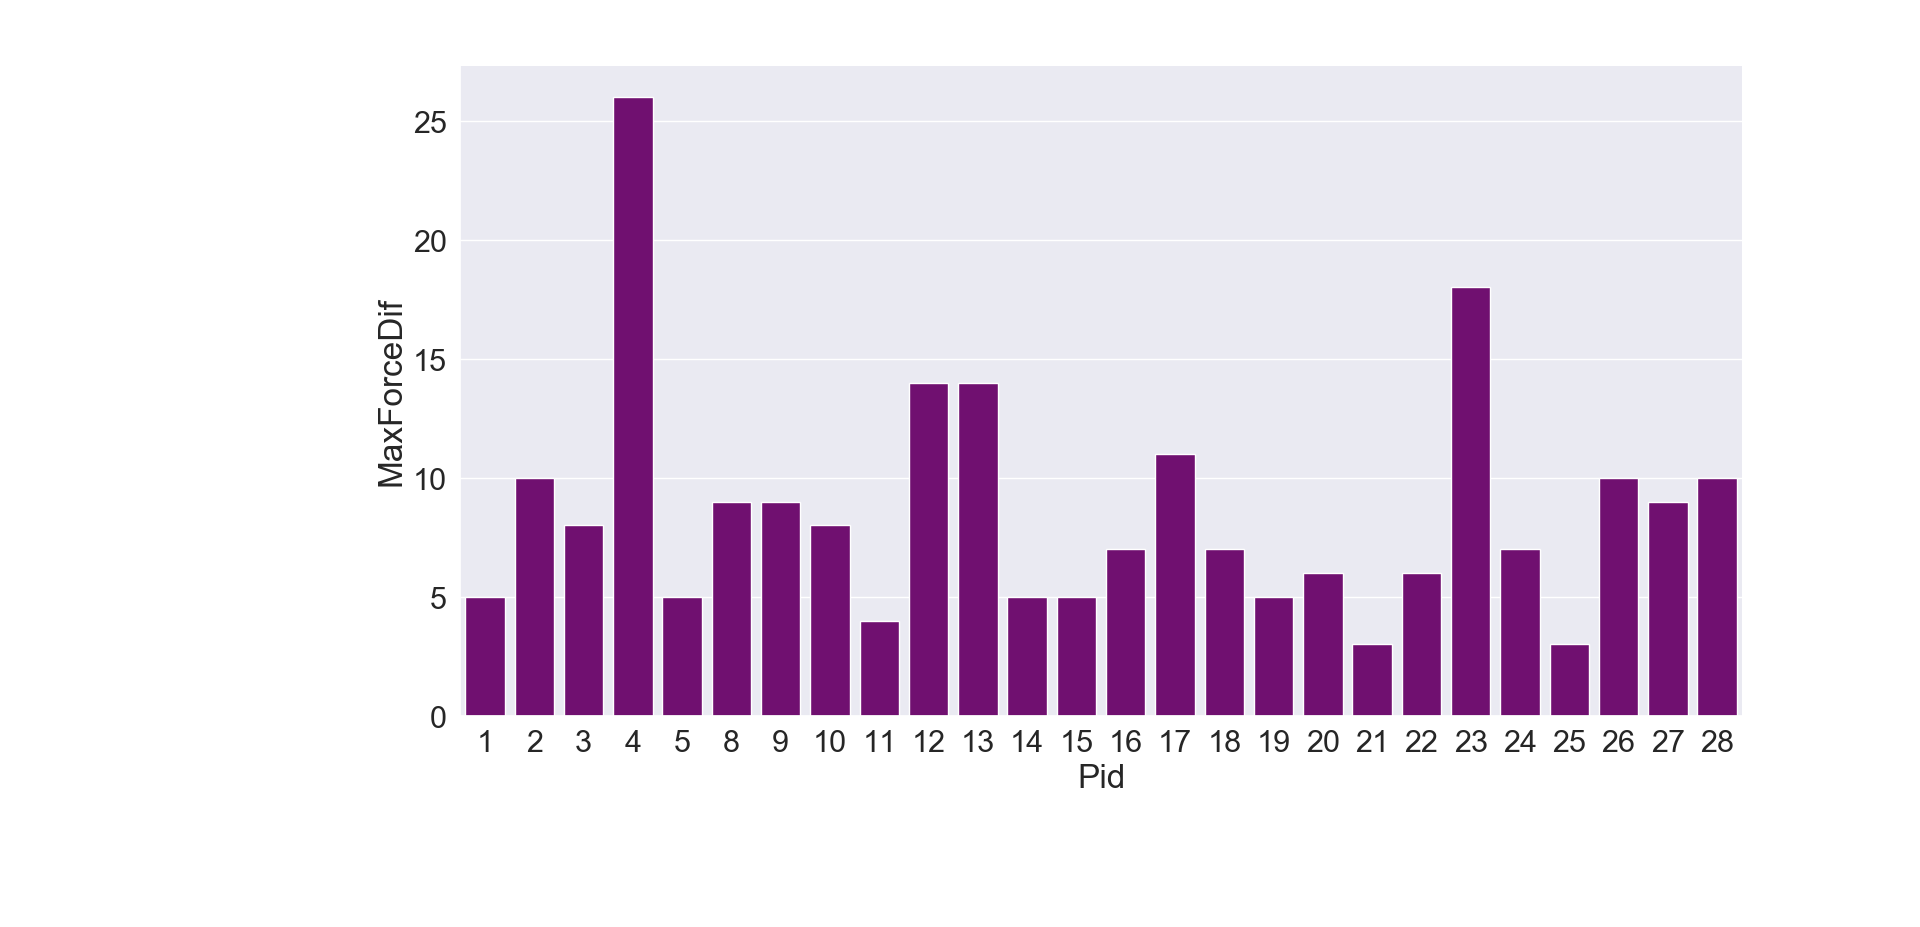
\includegraphics[scale=0.7]{Files/Plots/max_force_dif.png}
 \caption{Maximum force difference per participant.}
\label{fig:forceDif}
\end{figure} 

Max pull difference between trials at  participant 4 =26

mean of maximum differences = 8.615384615384615

standard dev= 4.949958288736037

 \clearpage   

\subsubsection{Perceived Pull and Challenge}
\label{subsubsection:ppullChallenge}
%%%%%%%%%%%%%%%%%%%%%%%%%%%%%%%%%%%%%%%%
%               CHALLENGE ppull counts
%%%%%%%%%%%%%%%%%%%%%%%%%%%%%%%%%%%%%%%
  
\begin{figure}[H]
\centering
\captionsetup{justification=centering,margin=0.1cm}
\hspace{-20mm}
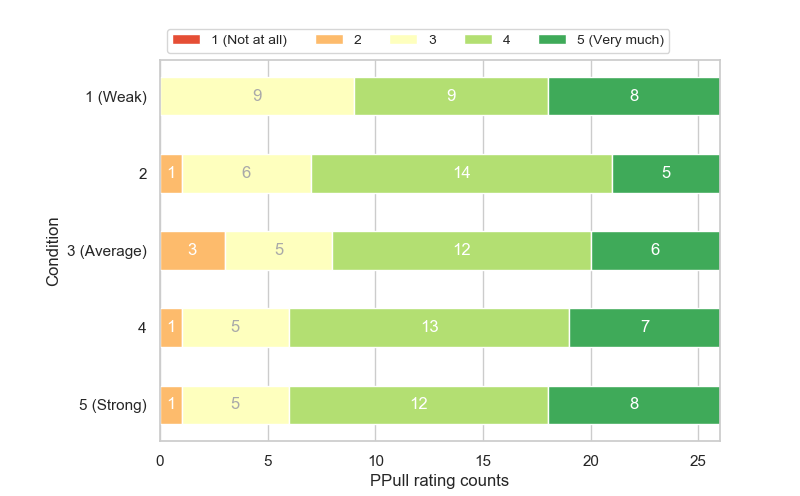
\includegraphics[scale=0.7]{Files/Plots/ppull_by_condition_count_stacked.png}
\caption{Count of perceived pull ratings by condition.}
\label{fig:ppullStacked}
\end{figure}
\vspace{-5mm}

\begin{figure}[H]
\captionsetup{justification=centering,margin=0.1cm}
 \centering
 \hspace{-20mm}
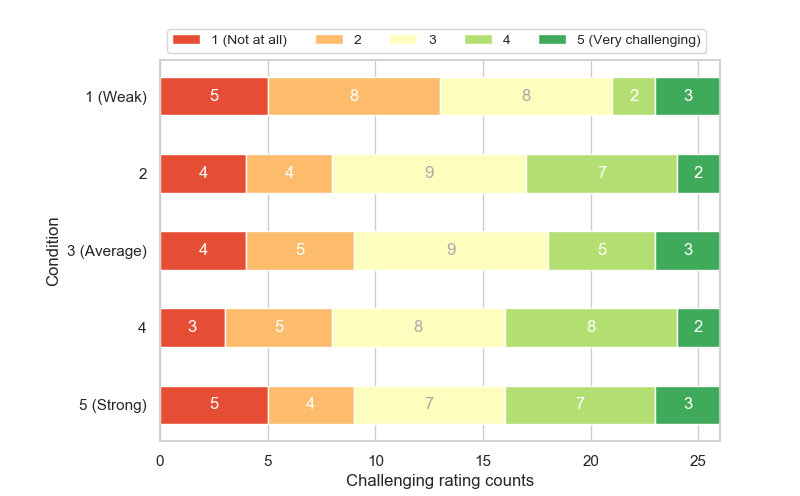
\includegraphics[scale=0.7]{Files/Plots/challenge_by_condition_count_staked.png}
\caption{Count of challenge ratings by condition.}
\label{fig:challengeStacked}
\end{figure}

\clearpage
Above in figures \ref{fig:ppullStacked} and 
\ref{fig:challengeStacked} we present an overview of the 5-point ratings by condition. In section \ref{subsection:heatmap} we show the total ratings for each participant for perceived pull (\ref{fig:ppullHeatmap}) and challenge (\ref{fig:challengeHeatmap}).

%%%%%%%%%%%%%%%%%%%%%%%%%%%%%%%%%%%%%%%%
%               CHALLENGE
%%%%%%%%%%%%%%%%%%%%%%%%%%%%%%%%%%%%%%%
    
\begin{figure}[H]
 \begin{subfigure}[b]{0.5\textwidth}
     \centering
     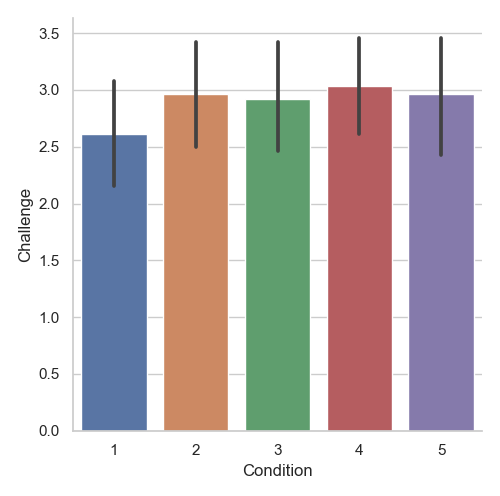
\includegraphics[scale=0.5]{Files/Plots/challenge_by_condition_mean.png}
     \caption{Mean challenge by condition.}
     \label{fig:meanChal}
 \end{subfigure}
  \begin{subfigure}[b]{0.5\textwidth}
     \centering
     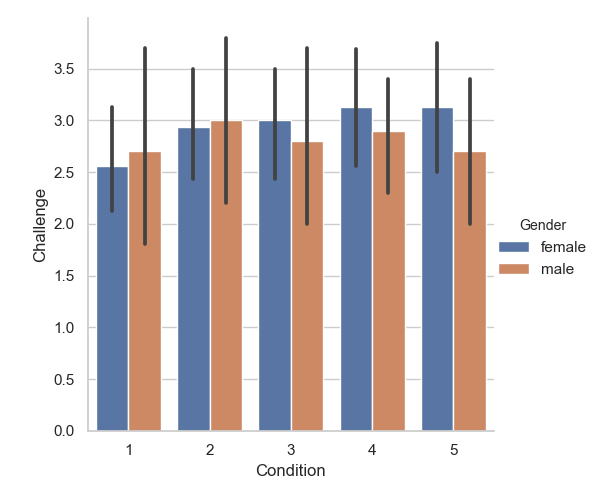
\includegraphics[scale=0.5]{Files/Plots/challenge_by_condition_mean_gen.png}
     \caption{Mean challenge by condition gendered.}
     \label{fig:fig:meanChalGen}
 \end{subfigure}
     \caption{Mean challenge by condition, and by gender. Lines on bars denote confidence intervals.}
    \label{fig:chalByCond}
\end{figure}

\begin{figure}[H]
 \begin{subfigure}[b]{0.5\textwidth}
     \centering
     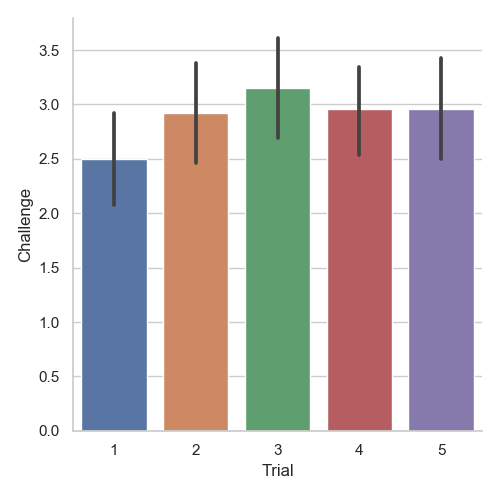
\includegraphics[scale=0.5]{Files/Plots/challenge_by_trial_mean.png}
     \caption{Mean challenge by trial.}
     \label{fig:meanChal}
 \end{subfigure}
  \begin{subfigure}[b]{0.5\textwidth}
     \centering
     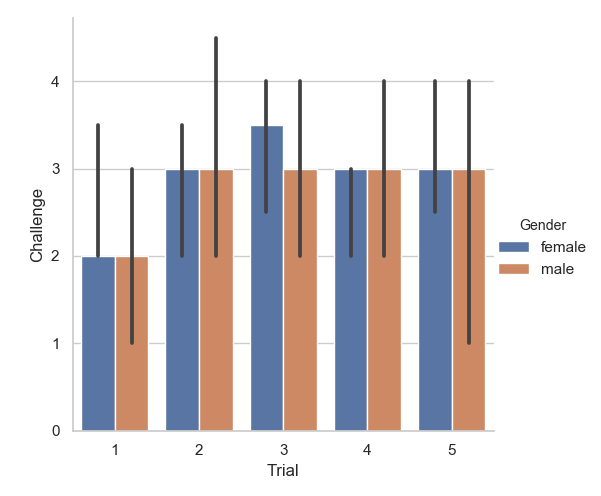
\includegraphics[scale=0.5]{Files/Plots/challenge_by_trial_mean_gen.png}
     \caption{Mean challenge by trial gendered.}
     \label{fig:fig:meanChalGen}
 \end{subfigure}
     \caption{Mean challenge by trial, and by gender. Lines on bars denote confidence intervals.}
    \label{fig:chalByCond}
\end{figure}

\begin{figure}[H]
 \begin{subfigure}[b]{0.5\textwidth}
     \centering
     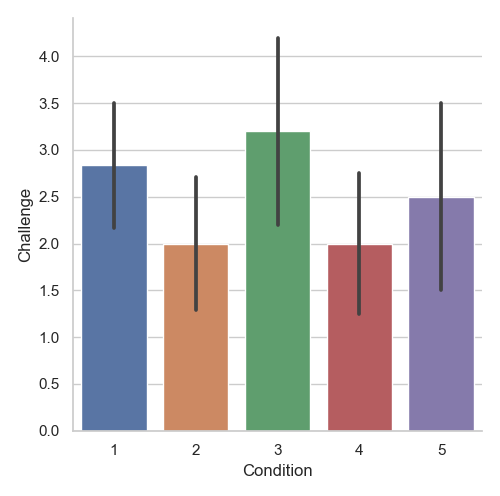
\includegraphics[scale=0.5]{Files/Plots/challenge_first_trial.png}
     \caption{Mean challenge for 1st trial.}
     \label{fig:meanChal1st}
 \end{subfigure}
  \begin{subfigure}[b]{0.5\textwidth}
     \centering
     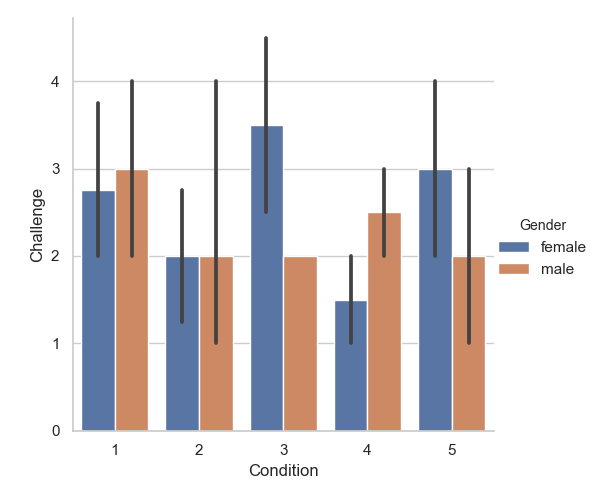
\includegraphics[scale=0.5]{Files/Plots/challenge_first_trial_gen.png}
     \caption{Mean challenge for 1st trial gendered.}
     \label{fig:meanChalGen1st}
 \end{subfigure}
  \begin{subfigure}[b]{0.5\textwidth}
     \centering
     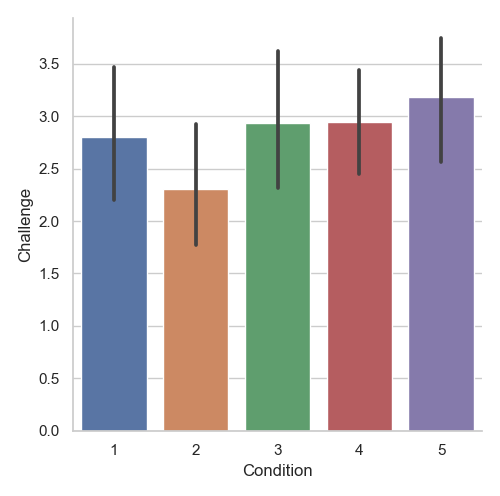
\includegraphics[scale=0.5]{Files/Plots/challenge_first_3_trials.png}
     \caption{Mean challenge for first 3 trials.}
     \label{fig:meanChal3rd}
 \end{subfigure}
     \begin{subfigure}[b]{0.5\textwidth}
     \centering
     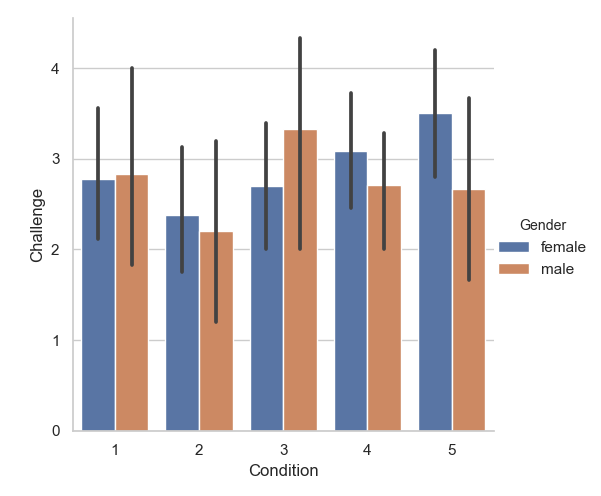
\includegraphics[scale=0.5]{Files/Plots/challenge_first_3_trials_gen.png}
     \caption{Mean challenge for first 3 trials gendered.}
     \label{fig:meanChalGen3rd}
 \end{subfigure}
     \caption{Mean challenge by condition, and by gender for first and first three trials. Lines on bars denote confidence intervals.}
    \label{fig:Chal1st3rd}
\end{figure}

%%%%%%%%%%%%%%%%%%%%%%%%%%%%%%%%%%%%%%%%
%               ppull
%%%%%%%%%%%%%%%%%%%%%%%%%%%%%%%%%%%%%%%
    
\begin{figure}[H]
 \begin{subfigure}[b]{0.5\textwidth}
     \centering
     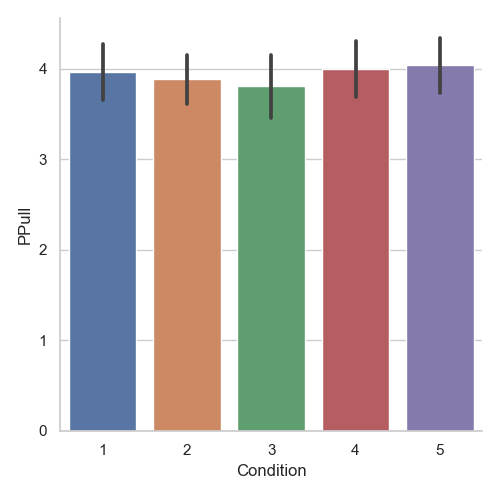
\includegraphics[scale=0.5]{Files/Plots/ppull_by_condition_mean.png}
     \caption{Mean perceived pull by condition.}
     \label{fig:meanPPullCond}
 \end{subfigure}
  \begin{subfigure}[b]{0.5\textwidth}
     \centering
     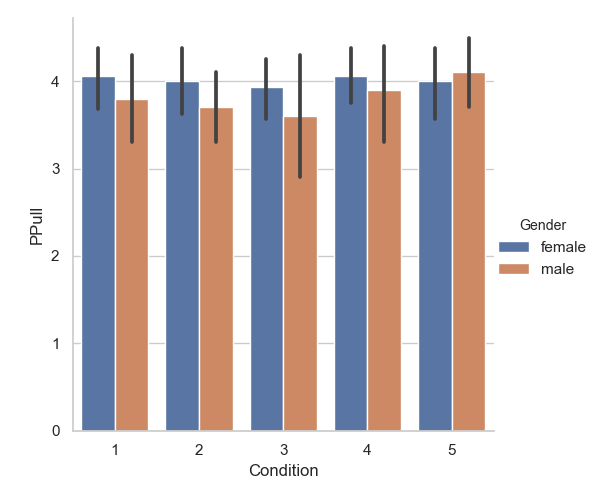
\includegraphics[scale=0.5]{Files/Plots/ppull_by_condition_median_gen.png}
     \caption{Mean ppull by condition gendered.}
     \label{fig:fig:meanPPullGenCond}
 \end{subfigure}
     \caption{Mean perceived pull by condition, and by gender. Lines on bars denote confidence intervals.}
    \label{fig:ppullByCond}
\end{figure}

\begin{figure}[H]
 \begin{subfigure}[b]{0.5\textwidth}
     \centering
     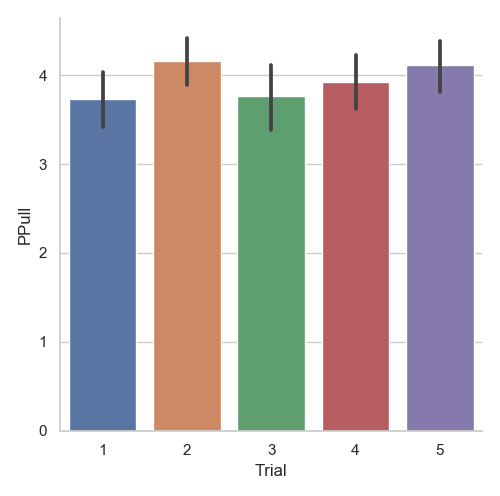
\includegraphics[scale=0.5]{Files/Plots/ppull_by_trial_mean.png}
     \caption{Mean perceived pull by trial.}
     \label{fig:meanPpullTrial}
 \end{subfigure}
  \begin{subfigure}[b]{0.5\textwidth}
     \centering
     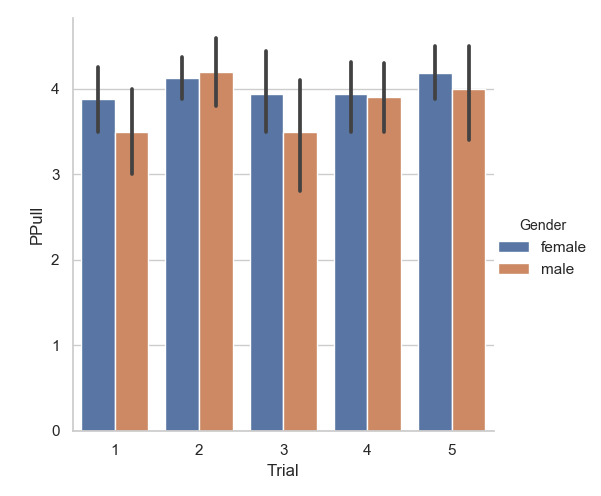
\includegraphics[scale=0.5]{Files/Plots/ppull_by_trial_mean_gen.png}
     \caption{Mean perceived pull by trial gendered.}
     \label{fig:meanPPullGenTrial}
 \end{subfigure}
     \caption{Mean perceived pull by trial, and by gender. Lines on bars denote confidence intervals.}
    \label{fig:ppullByTrial}
\end{figure}

\begin{figure}[H]
 \begin{subfigure}[b]{0.5\textwidth}
     \centering
     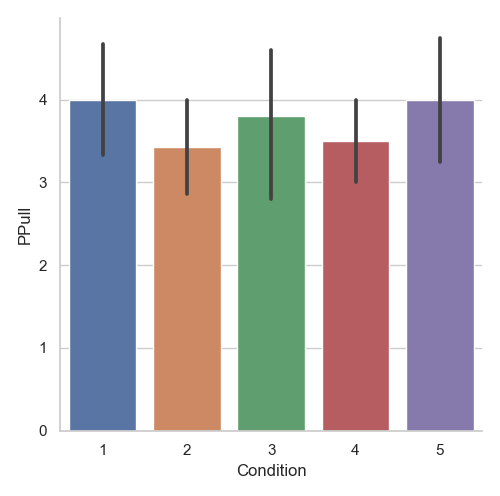
\includegraphics[scale=0.5]{Files/Plots/ppull_first_trial.png}
     \caption{Mean perceived pull for 1st trial.}
     \label{fig:meanPPull1st}
 \end{subfigure}
  \begin{subfigure}[b]{0.5\textwidth}
     \centering
     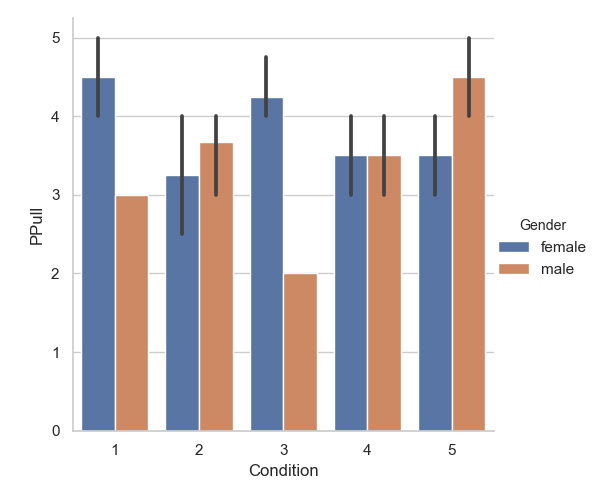
\includegraphics[scale=0.5]{Files/Plots/ppull_first_trial_gen.png}
     \caption{Mean ppull for 1st trial gendered.}
     \label{fig:meanPPullGen1st}
 \end{subfigure}
  \begin{subfigure}[b]{0.5\textwidth}
     \centering
     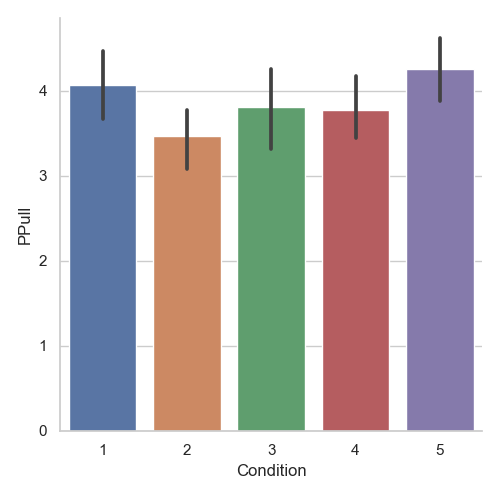
\includegraphics[scale=0.5]{Files/Plots/ppull_first_3_trials.png}
     \caption{Mean ppull for first 3 trials.}
     \label{fig:meanPPull3rd}
 \end{subfigure}
     \begin{subfigure}[b]{0.5\textwidth}
     \centering
     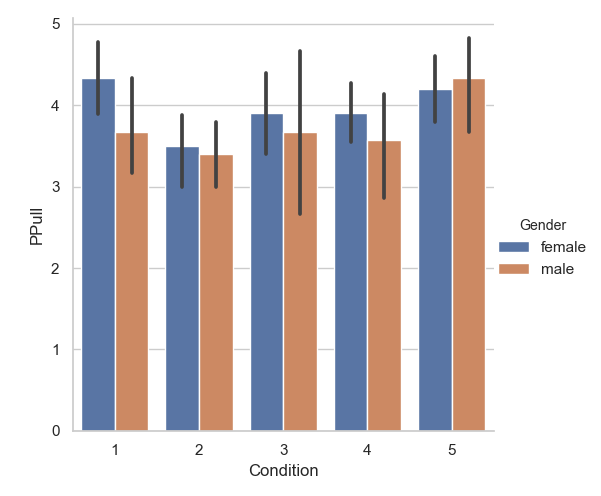
\includegraphics[scale=0.5]{Files/Plots/ppull_first_3_trials_gen.png}
     \caption{Mean ppull for first 3 trials gendered.}
     \label{fig:meanPPullGen3rd}
 \end{subfigure}
     \caption{Mean perceived pull by condition, and by gender for first and first three trials. Lines on bars denote confidence intervals.}
    \label{fig:PPull1st3rd}
\end{figure}


\subsubsection{Rope Ownership and Realism}
\label{subsubsection:ropeOwnRealism}
%%%%%%%%%%%%%%%%%%%%%%%%%%%%%%%%%%%%%%%%
%               rope ownership
%%%%%%%%%%%%%%%%%%%%%%%%%%%%%%%%%%%%%%%


\begin{figure}[H]
 \begin{subfigure}[b]{0.5\textwidth}
     \centering
     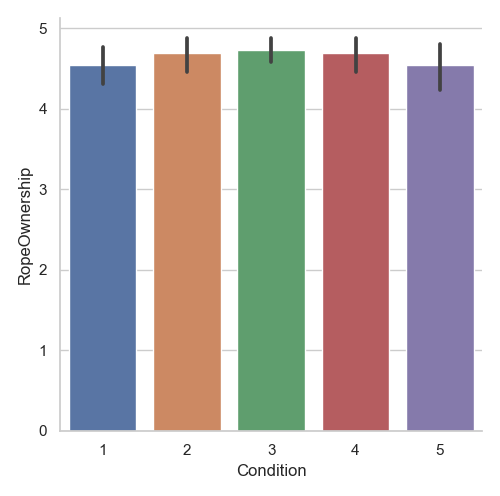
\includegraphics[scale=0.5]{Files/Plots/ropeOwnership_by_condition.png}
     \caption{Mean rope ownership by condition.}
     \label{fig:ropeOwnCond}
 \end{subfigure}
  \begin{subfigure}[b]{0.5\textwidth}
     \centering
     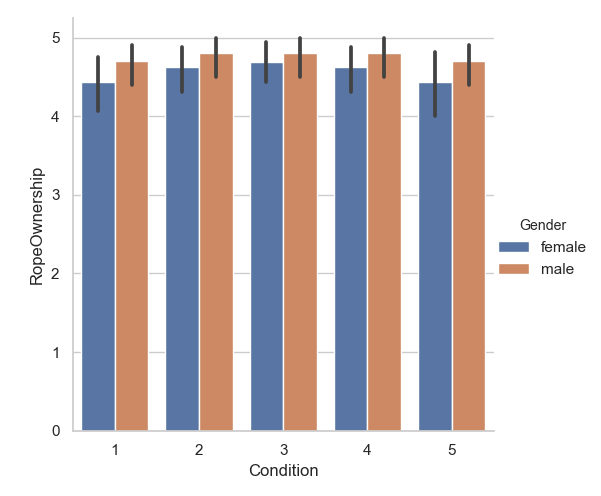
\includegraphics[scale=0.5]{Files/Plots/ropeOwnership_by_condition_gen.png}
     \caption{Mean rope ownership by condition gendered.}
     \label{fig:ropeOwnCondGend}
 \end{subfigure}
  \begin{subfigure}[b]{0.5\textwidth}
     \centering
     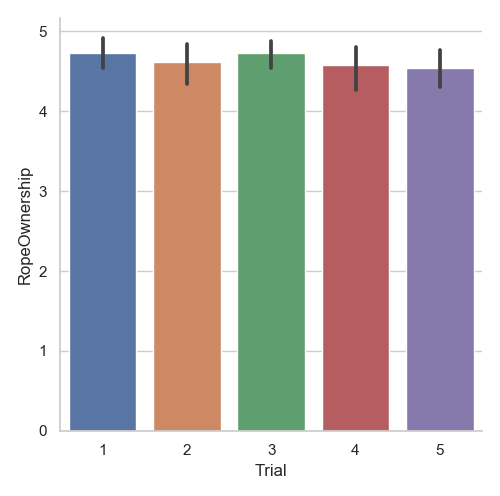
\includegraphics[scale=0.5]{Files/Plots/ropeOwnership_by_trial.png}
     \caption{Mean rope ownership by trial.}
     \label{fig:ropeOwnTrial}
 \end{subfigure}
     \begin{subfigure}[b]{0.5\textwidth}
     \centering
     \includegraphics[scale=0.5]{Files/Plots/ropeOwnership_by_trial_gen.png}
     \caption{Mean rope ownership by trial gendered.}
     \label{fig:ropeOwnTrialGen}
 \end{subfigure}
     \caption{Mean rope ownership by condition, trial and by gender. Lines on bars are confidence intervals.}
    \label{fig:ropeOwn}
\end{figure}


%%%%%%%%%%%%%%%%%%%%%%%%%%%%%%%%%%%%%%%%
%               rope realism
%%%%%%%%%%%%%%%%%%%%%%%%%%%%%%%%%%%%%%%

\begin{figure}[H]
 \begin{subfigure}[b]{0.5\textwidth}
     \centering
     \includegraphics[scale=0.5]{Files/Plots/ropeRealism_by_condition.png}
     \caption{Mean rope realism by condition.}
     \label{fig:ropeRealCond}
 \end{subfigure}
  \begin{subfigure}[b]{0.5\textwidth}
     \centering
     \includegraphics[scale=0.5]{Files/Plots/ropeRealism_by_condition_gen.png}
     \caption{Mean rope realism by condition gendered.}
     \label{fig:ropeRealCondGend}
 \end{subfigure}
  \begin{subfigure}[b]{0.5\textwidth}
     \centering
     \includegraphics[scale=0.5]{Files/Plots/ropeRealism_by_trial.png}
     \caption{Mean rope realism by trial.}
     \label{fig:ropeRealTrial}
 \end{subfigure}
     \begin{subfigure}[b]{0.5\textwidth}
     \centering
     \includegraphics[scale=0.5]{Files/Plots/ropeOwnership_by_trial_gen.png}
     \caption{Mean rope realism by trial gendered.}
     \label{fig:ropeRealTrialGen}
 \end{subfigure}
     \caption{Mean rope realism by condition, trial and by gender. Lines on bars are confidence intervals.}
    \label{fig:ropeRealism}
\end{figure}
\clearpage

\subsubsection{Post-experimental Survey Results}

In the following, bar lines denotes standard deviation.

%%%%%%%%%%%%%%%%%%%%%%%%%%%%%%%%%%%%%%%%
%           misc all    %%%%%%%%%%%%%%%%%%%%%%%%%%%%%%%%%%%%%%%

\begin{figure}[H]
 \centering
 \includegraphics[scale=0.5]{Files/Plots/gaze_plots.png}
 \caption{Percent participants gazed at objects during the whole experiment duration. }
\label{fig:gazePie}
\end{figure}

We did not have eye tracking, however we used the midpoint of the headset to estimate what objects participants were looking at.

\begin{figure}[H]
 \centering
 \includegraphics[scale=0.5]{Files/Plots/misc_all_mean.png}
 \caption{Total mean co-presence, presence and ownership ratings.}
\label{fig:miscAll}
\end{figure}

Co-presence   Presence       Ownership
3.538462         3.515385       3.698718
0.99604742    0.97849661    1.26804853


\begin{figure}[H]
\begin{subfigure}[b]{0.5\textwidth}
 \centering
 \includegraphics[scale=0.4]{Files/Plots/misc_all_mean_f.png}
 \caption{Females mean ratings. }
 \label{fig:miscAllFemales}
 \end{subfigure}
\begin{subfigure}[b]{0.5\textwidth}
 \centering
 \includegraphics[scale=0.4]{Files/Plots/misc_all_mean_m.png}
 \caption{Males mean ratings.}
 \label{fig:miscAllMales}
 \end{subfigure}
 \caption{Total mean co-presence, presence and ownership ratings by gender. }
\label{fig:miscAllGendered}
\end{figure}

%%%%%%%%%%%%%%%%%%%%%%%%%%%%%%%%%%%%%%%%
%             copresence
%%%%%%%%%%%%%%%%%%%%%%%%%%%%%%%%%%%%%%%

\begin{figure}[H]
\hspace{-15mm}
\begin{subfigure}[b]{0.3\textwidth}
 \centering
 \includegraphics[scale=0.33]{Files/Plots/copresence_mean.png}
 \caption{Total mean ratings. }
 \label{fig:copresAll}
 \end{subfigure}
 \hspace{10mm}
\begin{subfigure}[b]{0.3\textwidth}
 \centering
 \includegraphics[scale=0.33]{Files/Plots/copresence_mean_f.png}
 \caption{Females mean ratings.}
 \label{fig:copresFemale}
 \end{subfigure}
  \hspace{10mm}
 \begin{subfigure}[b]{0.3\textwidth}
 \centering
 \includegraphics[scale=0.33]{Files/Plots/copresence_mean_m.png}
 \caption{Males mean ratings.}
 \label{fig:copresMale}
 \end{subfigure}
 \caption{\textbf{Co-presence} ratings, by mean and gender.}
\label{fig:coAll}
\end{figure}

Copresence mean
0    Q1  My opponents were intensely involved in our in...  3.461538
1    Q2  To what extent did you feel able to assess you...  3.038462
2    Q3  To what extent was this like you were in the s...  4.115385

Std
0    Q1  My opponents were intensely involved in our in...  0.859338
1    Q2  To what extent did you feel able to assess you...  1.076319
2    Q3  To what extent was this like you were in the s...  0.765607


  index                                                  q    0
0    Q1  My opponents were intensely involved in our in...  4.0
1    Q2  To what extent did you feel able to assess you...  3.0
2    Q3  To what extent was this like you were in the s...  4.0

%%%%%%%%%%%%%%%%%%%%%%%%%%%%%%%%%%%%%%%%
%             presence
%%%%%%%%%%%%%%%%%%%%%%%%%%%%%%%%%%%%%%%
\begin{figure}[H]
\hspace{-15mm}
\begin{subfigure}[b]{0.3\textwidth}
 \centering
 \includegraphics[scale=0.33]{Files/Plots/presence_mean_ratings.png}
 \caption{Total mean ratings. }
 \label{fig:presAll}
 \end{subfigure}
 \hspace{10mm}
\begin{subfigure}[b]{0.3\textwidth}
 \centering
 \includegraphics[scale=0.33]{Files/Plots/presence_mean_ratings_f.png}
 \caption{Females mean ratings.}
 \label{fig:presFemale}
 \end{subfigure}
  \hspace{10mm}
 \begin{subfigure}[b]{0.3\textwidth}
 \centering
 \includegraphics[scale=0.33]{Files/Plots/presence_mean_ratings_m.png}
 \caption{Males mean ratings.}
 \label{fig:presMale}
 \end{subfigure}
 \caption{\textbf{Presence} ratings, by mean and gender.}
\label{fig:presAll}
\end{figure}


mean

0    Q1  How aware were you of the real world surroundi...  2.692308
1    Q2       How real did the virtual world seem to you?   3.384615
2    Q3  How much did your experience in the virtual en...  3.269231
3    Q4              I felt present in the virtual space.   4.115385
4    Q5  In the computer generated world I had a sense ...  4.115385


Std
  index                                                  q         0
0    Q1  How aware were you of the real world surroundi...  1.010712
1    Q2       How real did the virtual world seem to you?   0.752432
2    Q3  How much did your experience in the virtual en...  1.002305
3    Q4              I felt present in the virtual space.   0.652805
4    Q5  In the computer generated world I had a sense ...  0.652805


median
  index                                                  q    0
0    Q1  How aware were you of the real world surroundi...  3.0
1    Q2       How real did the virtual world seem to you?   3.0
2    Q3  How much did your experience in the virtual en...  3.0
3    Q4              I felt present in the virtual space.   4.0
4    Q5  In the computer generated world I had a sense ...  4.0



%%%%%%%%%%%%%%%%%%%%%%%%%%%%%%%%%%%%%%%%
%             ownership
%%%%%%%%%%%%%%%%%%%%%%%%%%%%%%%%%%%%%%%
\begin{figure}[H]
\hspace{-15mm}
\begin{subfigure}[b]{0.3\textwidth}
 \centering
 \includegraphics[scale=0.33]{Files/Plots/ownership_mean.png}
 \caption{Total mean ratings. }
 \label{fig:ownAll}
 \end{subfigure}
 \hspace{10mm}
\begin{subfigure}[b]{0.3\textwidth}
 \centering
 \includegraphics[scale=0.33]{Files/Plots/ownership_mean_ratings_f.png}
 \caption{Females mean ratings.}
 \label{fig:ownFemale}
 \end{subfigure}
  \hspace{10mm}
 \begin{subfigure}[b]{0.3\textwidth}
 \centering
 \includegraphics[scale=0.33]{Files/Plots/ownership_mean_ratings_m.png}
 \caption{Males mean ratings.}
 \label{fig:ownMale}
 \end{subfigure}
 \caption{\textbf{Arm ownership} ratings, by mean and gender.}
\label{fig:ownAll}
\end{figure}


  index                                                  q         0
0    Q1  I felt as if the virtual arm moved just like I...  3.807692
1    Q2  I expected the virtual arm to react in the sam...  4.538462
2    Q3  I felt that the interaction with the environme...  3.692308
3    Q4          I felt like I controlled the virtual arm.  4.346154
4    Q5  I felt as if the virtual arm was part of my body.  3.923077
5    Q6   I felt as if the virtual arm was someone else’s.  1.884615


  index                                                  q         0
0    Q1  I felt as if the virtual arm moved just like I...  1.200641
1    Q2  I expected the virtual arm to react in the sam...  0.508391
2    Q3  I felt that the interaction with the environme...  0.928191
3    Q4          I felt like I controlled the virtual arm.  0.845804
4    Q5  I felt as if the virtual arm was part of my body.  1.016782
5    Q6   I felt as if the virtual arm was someone else’s.  1.032547



Out[51]: 
  index                                                  q    0
0    Q1  I felt as if the virtual arm moved just like I...  4.0
1    Q2  I expected the virtual arm to react in the sam...  5.0
2    Q3  I felt that the interaction with the environme...  4.0
3    Q4          I felt like I controlled the virtual arm.  5.0
4    Q5  I felt as if the virtual arm was part of my body.  4.0
5    Q6   I felt as if the virtual arm was someone else’s.  2.0



\clearpage

\subsubsection{Post-experimental Qualitative Feedback}



Contrast isolated effect: If hands were too offseted for participants it decreased realism and it was more salient because the other elements in vr were seen as highly realistic - p1 

- person said they saw a strong guy and expected them to pull harder so they pulled less to feel it part 23 
-2 outliers where participants pulled too hard and they adjusted their strategy for that 



- holding the rope makes it feel more real
-ownership higher because of holding the rope


Inconsistencies in pulling despite qualitative feedback
I was expecting him to pull stronger so i pulled less to feel that
[reffering to seeing a stronger looking character] Okay… I should pull stronger  [...] it’s a natural response. [....OR IS  IT?]
Muddy plots express variability of human behavior - they were testing the machine
Various assumptions and reasoning for choosing answers especially for Challenge
I can't move them so it’s very challenging
Assumptions may change during the experiment depending on feedback of system



\subsection{Discussion}
\subsubsection{Appearance Ratings}
The ratings for female avatars for the VR tug-of-war were inconsistent with our results from the survey. There were several downsides when designing the female agents (detailed in section \ref{section:AgentDesign}) which lead to females being perceived overall as less strong and intimidating, even in the survey. One difference between the 2 studies is that participants playing tug-of-war could see the full body of the avatar in VR as well. On the other hand, participants filling in the survey only saw their thumbnails. The resolution of the headset could also impair the ability of people seeing the avatars very clearly. One participant mentioned that she would have liked to see the females with hair. It is possible the lack of hair on females might have put off participants instead of making strength cues more salient


\subsection{Limitations}
- spring absorbs force a participant stretched the spring too much and it was replaced\\
- force meter accuracy for the digital display
- person error prone?
-resolution and realism all had same movements but varying so many things would allow less control over the independent variables research wise, it would be difficult to establish causation,//
-ppl unsure about pulling the first round and there is some effect//
- force got maxim for whatever minimum amount of time other strategies can be used to measure with a force meter that is not digital - like the average value across all that time, the longest value for how many seconds. etc.
- there could be some effect that people held medium values for longer idk
-challenge - what is challenging what they rated with if they rated it by looks then it is bad. MMaking it implicit and explicit has advantages and disadvantages. For example cognitive load focusing only on the pull ...\\
-change ratings allow and mention some did some not

0-The downside of this is that some participants mentioned they experience cognitive load as they were trying not to move their legs during the pulls. They were focusing on that instead of focusing on pulling as hard as they can. To solve this, we can use a set up in which the ropes are tied to walling.

-participants misbehave pilot pilot to design the experiment against misuse